\documentclass{kththesis}

%\usepackage{csquotes} % Recommended by biblatex
\usepackage[style=numeric,sorting=none,backend=biber,citestyle=verbose]{biblatex}
%\addbibresource{references.bib} % The file containing our references, in BibTeX format

\title{Quality Assesment of OpenStreetMap Footpath Data for 3D City Recreation}
\alttitle{Kvalitetiv undersökning av OpenStreetMaps gångvägsdata för stadsmodellering i 3D}
\author{Alexander Hjelm}
\email{aljhelm@kth.se}
\supervisor{Christopher Peters}
\examiner{Jonas Beskow}
%\hostcompany{Företaget AB} % Remove this line if the project was not done at a host company
\programme{Master in Computer Science}
\school{School of Electrical Engineering and Computer Science}
\date{\today}

\usepackage[english]{babel}
\usepackage[utf8]{inputenc}
\usepackage{amsmath}
\usepackage{graphicx}
\usepackage[colorinlistoftodos]{todonotes}
\usepackage{float}
\usepackage{hyperref}
\usepackage{multicol}
\usepackage[ruled,vlined]{algorithm2e}
\usepackage{caption}

\setlength\parindent{0pt}
\setlength{\parskip}{1em}
\setcounter{tocdepth}{2}

% Uncomment the next line to include cover generated at https://intra.kth.se/kth-cover?l=en
% \kthcover{kth-cover.pdf}

\begin{document}

% Frontmatter includes the titlepage, abstracts and table-of-contents
\frontmatter

\titlepage

\begin{abstract}
Modeling cities in 3D has long been a topic of interest in field of computer graphics.
It is often desirable to recreate real-world cities in 3D applications such as urban design software and video games, and the topic of 3D city reproduction comes with its own set of unique challenges.
So far there have been a lot of research in modelling of 3D road networks, but these projects have often focused on the road networks designated for cars and public transit, and seldom on pedestrian footpaths.

This project assesses the feasibility of reconstructing a city from OpenStreetMap (OSM) road and building data, and will focus on the feasibility of including pedestrian footpaths, by examining how common it is that these footpaths collide with other map features.
In the collision detection process, the margin of error has been taken as the positional error in the OSM dataset, which has been obtained by comparing OSM data to a dataset with a known accuracy.

It was found that footpaths were less problematic than other road types (primary, secondary, residential), in terms of feature collisions, and thus should pose no more problems in 3D city reproduction than other road types.
The report concludes with a scientific study of the field of 3D city reproduction. It serves to give an overview of the challenges in the field and place the study and findings of this project in a broader scientific context. 
\end{abstract}

\begin{otherlanguage}{swedish}
\begin{abstract}
Haha, He-Man! There is no possible way that you feeble-brained barbarian and your furball mount can foil my plan this time. With the ancient power at my command I shall doom this kingdom to crumble in meager ashes and.. Oh shit, he has run off with the crystal skull hasn't he? Damn you He-Man!!!

\end{abstract}
\end{otherlanguage}

\tableofcontents

% Mainmatter is where the actual contents of the thesis goes
\mainmatter

\chapter{Introduction}

\begin{figure}[H]
    \centering
    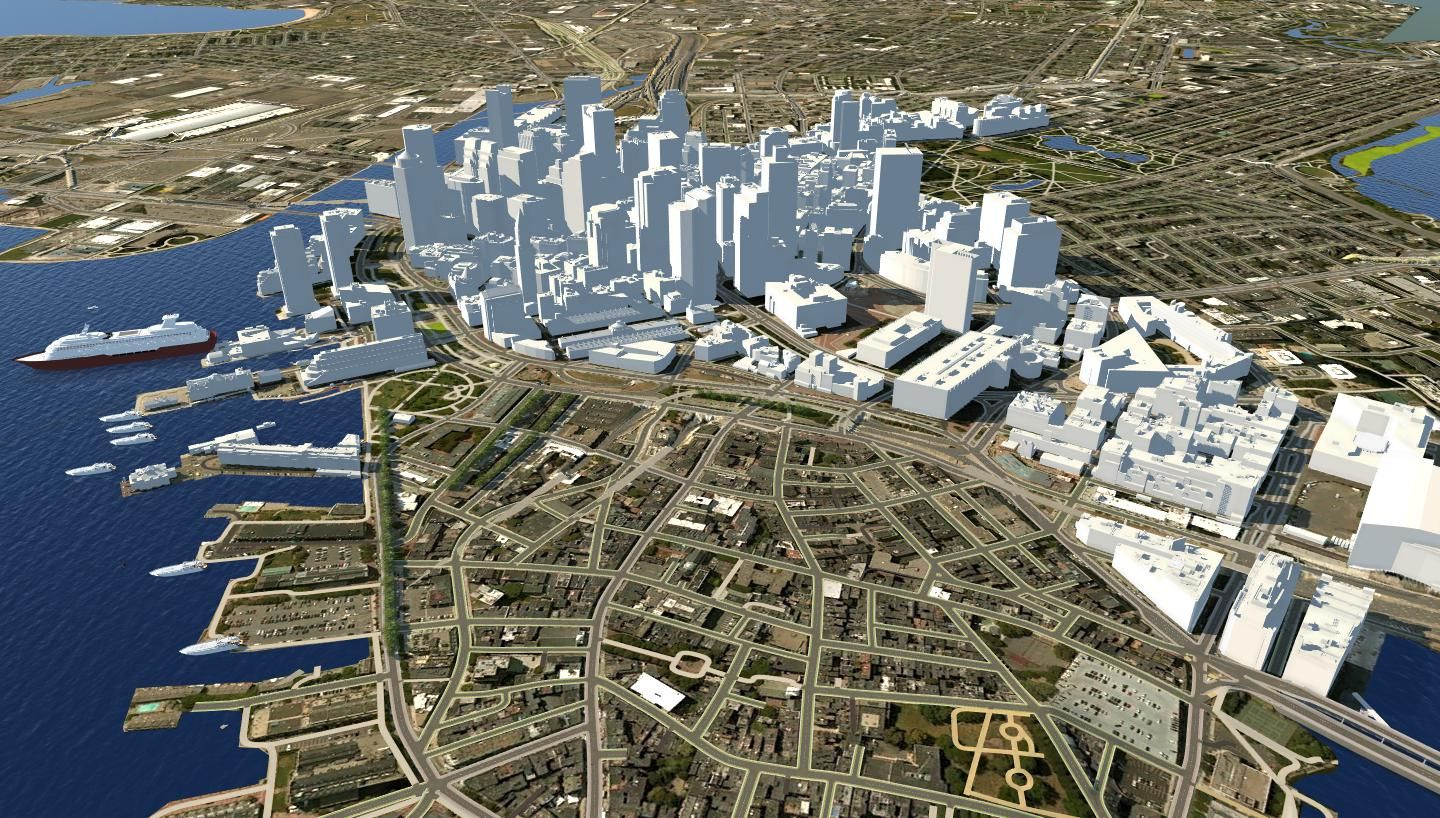
\includegraphics[width=\textwidth,height=0.5\textheight,keepaspectratio]{img_virtual_city}
    \caption{Real-world cities are complex collections of buildings, blocks and road networks that interconnect them all. Creating 3D virtual cities using methods of procedual generation is an emerging research field that comes with its own set of challenges. This project deals with generating virtual cities from OpenStreetMap data, and the technical challenges therein.}
    \label{fig:virtual-city}
\end{figure}

This project assesses the feasibility of reconstructing a city from OpenStreetMap (OSM) road and building data, and will focus on the feasibility of including pedestrian footpaths, by focusing on OSM road and building data in the Stockholm metropolitan area.

Virtual cities has in recent years been a popular research topic in the field of computer visualization.
The idea of recreating real world cities in 3D applications has a growing number of applications, including visualization and modelling, urban planning and architecture, as well as entertainment in the form of video games and 3D animation.
Traditionally, modelling virtual cities is a labour-intensive and time-consuming task.
However, in recent years there has been major research work in the field of procedural content generation, meaning automatic or semi automatic generation of 3D models without the direct involvment of a 3D artist.
Such methods can indeed be used in the field of virtual city reproduction to reduce the labour required to reproduce accurate 3D representations of cities, but the field of procedual city reproduction comes with its own host of challenges.
Urban environments are typically dense and large, spanning a few to hundreds of square kilometers, and are influenced by variables that are hard to quantify, including land policies, government plans, population changes and transportation infrastructure.
\textbf{(Vanegas et al, 2010)}.

Cities consist of complex collections of buildings, blocks, parcels and neighbourhoods which are all interconnected via a street network, where individual streets can serve different types of traffic.
These features are commonly represented as geodata in map databases, and processed and organized into visualization-ready data by a Geographic Information System (GIS).
In practise, cities are often made up out of many square kilometers worth of geodata, and it would be highly labour intensive to recreate all the features in 3D.
Instead, procedural models for city reproduction instead rely on programmatic solutions for converting map data to 3D road and building models, and composing them to a 3D world that the designer may continue to fine-tweak through interfaces fo interactive editing.
At the very base of this process is the procedural layout of road networks in 3D,
\textbf{(Müller et al, 2006)}
and so far there have been a lot of research in modelling of 3D road networks, but these projects have often focused on the road networks designated for cars and public transit, as a part of the sustainable mobility paradigm and the topic of sustainable cities, particularily due to the interest in self-propelled cars.
The study of energy efficient mobility such as walking and cycling is only in its emerging phase. \textbf{(Stojanovski, 2019)}

\begin{figure}[H]
    \centering
    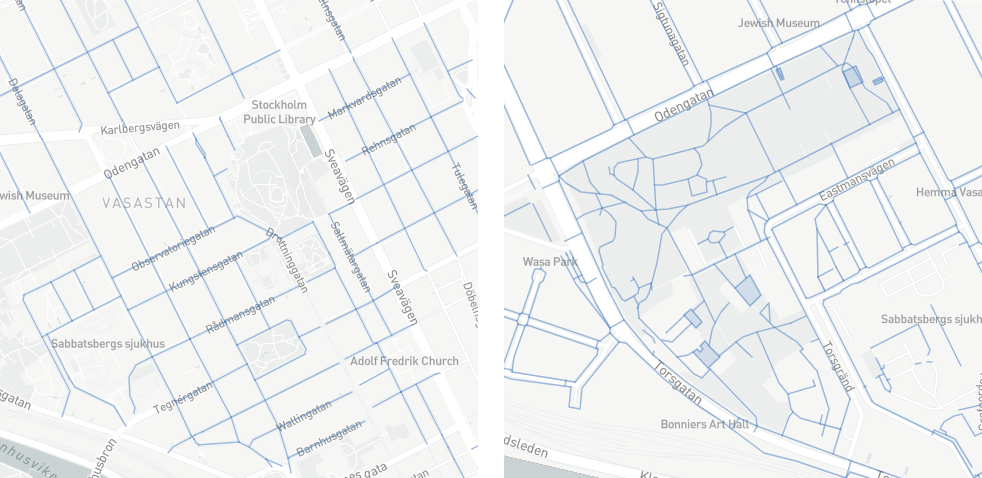
\includegraphics[width=\textwidth,height=0.5\textheight,keepaspectratio]{img_map_residential_footpath_compare}
    \caption{Example segments of the Stockholm metropolitan area with highlighted residential streets (left) and footpaths (right). Here can be seen the unique character of footpaths. Walkways in parks appear to grow much more organically, and pavements form rough grid systems with organic branches that bridge over city blocks.}
    \label{fig:residential-footpath-map}
\end{figure}

When it comes to the quality of available data, it turns out that in practise, 3D GIS datasets without errors are rare.
Among the most common errors are missing or invalid geometry, and invalid semantics.
However, \textbf{(Biljecki et al, 2016)} note that there are coming more and more sophisticated methods for automatically correcting the most common errors.
GIS validation and correction is only an emerging field of research.
and many such datasets were usually obtained years ago, and creating error-free datasets was neither possible due to the lack of validation techniques, nor a high priority.

A possible way of mitigating this problem is looking towards gathering geodata from volunteer-based geoservices such as OSM, where the temporal aspect of data accuracy is perhaps more assured by the crowd contribution nature.
There are already a few such services that use OSM data to generate 3D geodata visualizations for data visualization and video game applications.
A few prominent examples are Mantle
\footnote{Mantle homepage. Accessed 17-05-2020. https://www.mantle.tech/}
and Mapbox
\footnote{Mapbox homepage. Accessed 17-05-2020. https://www.mapbox.com/}.
Such services are however usually limited in the accuracy and type of data that they can provide.
While they can provide both builing footprints and road networks, they usually provide road data with no respect to overlap between features.
Collision between road meshes in 3D will lead to strange-looking mesh intersections and inaccuracies that modelers often want to avoid.
In particular, streets and roads designated for energy efficient mobility, such as footpaths, are much more organic and dense in their nature than main streets, and thus the risk of feature collision may be higher.

\section{Research question}

This project has dealt with the feasibility of including footpath data when generating 3D representations of OSM data, and preserving the integrity of the 3D road network, avoiding overlap and collision between road meshes.
The main contributions are as follows:

\begin{enumerate}
    \item The primary contribution is an \textbf{investigation into the rate of collision between map features in OSM}. How many roads of each type will collide with some other map feature once they have been given a geometrical width?
    \item The secondary contribution will be an \textbf{assesment of the geometrical precision of OSM data}. What is the positional accuracy of OSM map features compared to a reference map?
\end{enumerate}

For the primary contribution: the collision study, a program has taken an OSM dataset of the Stockholm area and assigned each road with standard withds according to swedish regulation.
It has then identified critical areas in the OSM dataset, where the paths are so wide that they collide with existing map features.
It has also identified how many of those areas can in theory be corrected by simple translation of the road vertices, without propagation of collision to other features.
Here, features are defined as the geometrical components that comprise the OSM map.
For the purpose of this report, features will refer mainly to roads and building footprints.
For the collision study, see sections 1.3.1 for an implementation overview, 4.2 for a detailed walkthrough of the program implementation, and 5.1 for the results.

For the secondary contribution: the geodata precision study, the positional accuracy will be estimated by comparing feature points between the OSM dataset and a reference dataset.
The positional accuracy will be needed to assess where road collisions occur and whether they can easily be corrected.
For the positional accuracy study, see sections 1.3.2 for an implementation overview, 4.1 for a walkthrough of the program implementation, and 5.2 for the results.

\section{Implementation overview}

\subsection{Assesment of geodata precision}

The geometrical precision study has been carried out in a number of steps that are all detailed below.
First a feature map was found, which mapped individual features between the OSM dataset and a reference dataset.
A program then took matching building pairs and extracted matching geometrical points after first simplifying the polygons using the Douglas-Peucker algorithm \textbf{(Douglas and Peucker, 1973)}.
Once a set of matching points has been found across the whole dataset, the average distance between them was taken as a measure of the positional accuracy.

Additionally, a number of auxillary calculations were neccessary for this study.
The estimated completeness of the OSM dataset (a measure of how many features are represented in both the OSM dataset and the reference dataset) was calculated as the relative difference in area of all building footprints, between the two datasets.
The completeness is needed to estimate the error boundary of the positional accuracy.
Additionally, the shape accuracy of the OSM dataset has also been calculated and graphed as an extra verification of the similarity between the datasets.

\subsection{Collision study}

The estimate of the positional error has was used to assess the integrity of the OSM Stockholm road network, by locating critical points where assigning standard widths to the roads would cause collision with other features, and evaluating how many of those points could be eliminated by making ajustments within the found margin of error.
For the purpose of the collision study, each road has been assigned a standard width that is in line with Swedish regulations, since in the OSM dataset, roads are represented as simple polylines, lacking width.
In a 3D representation however, it is crucial that each road object has a spacial width in order to be rendered and seen.
After the width assignment, a program has iterated over all features and calculated how many of them that overlap with any other feature, as well as the total length of the road polylines that is intersecting some other feature.
The program has then calculated how many of these colliding features that can be corrected by making adjustments that are within the positional accuracy of the OSM data (As obtained by the previous study in this report: Assessment of Geodata Precision).

\chapter{Methodology and evaluation}

\section{Evaluation metrics}

The primary study of the rate of collision between roads and other features, will serve to obtain the following three metrics:

\begin{enumerate}
    \item The number of road features that collide with any other feature (road or building).
    \item The number of road edges that intersect with any other building polygon or road polyline.
    \item The total length in meters of these edges will also be calculated as a measure of the total length of road.
\end{enumerate}

The road features will be categorized according to type, so that the rate of collisions between footpaths and other features can be compared to that of other road types.
OSM mainly makes the distinction between primary, secondary, residential and footpath roads, so this classification will also be used in this report.
The above features will be calculated for each road type separately by summing over each road feature of a certain type.
Following this, an algorithm will find the exact same metrics with regards to how many road features that can in theory be corrected by simple geometrical translation of their vertices.
This will also be preseneted in terms of the number of road features, the number of edges and the total length in meters of remaining colliding road.

The secondary study about geodata precision will primarily serve to obtain an estimate of the positional accuracy of the OSM dataset, in meters.
A number of auxillary metrics will be needed to estimate the domain of error on the positional accuracy, namely the feature completeness and shape accuracy of the OSM dataset.
The completeness of the OSM dataset will be taken as a the number of features are represented in both datasets, as a perentage of the total numer of features in the reference dataset.
Shape accuracy is a measure of polygon similarity that was obtained by comparing polygon turning function between matching features, feature by feature.
See section 5.3 for more details about the shape accuracy measure.

\section{Problem constraints}

In this study, when working with OSM geodata, the following assumptions have been made about the dataset to reduce the size of the problem domain:

\begin{enumerate}
    \item The program will not handle terrain features and altitude. It will be assumed that the road mesh can be projected on a flat 2D surface without feature intersection.
    \item It will be assumed that the city map consists of only arterial (primary) roads, secondary roads and footpaths.
    \item It will be assumed that the OSM dataset represents all roads as simple polylines, and building footprints as simple connected polygons. Any other features (such as squares, which are roads represented as polygons) will be omitted from the dataset.
    \item The road network is assumed to be a 2D simple graph. This means that any overlapping roads, such as tunnels and bridges that cross over street-level roads, will be eliminated from the dataset. Any self-connected nodes will also be eliminated from the dataset.
\end{enumerate}

\section{Quality criteria}

\textbf{(Haklay, 2010)} presents a comprehesive list of 8 accuracy classes when it comes to evaluating the quality of geographic information (van Oorts criteria)

\begin{itemize}
  \item Lineage. This is the historical aspect of the dataset, which concerns the collection process and evolution.
  \item Positional accuracy. This relates the coordinate value of an object in the database to the actual location of the ground in the real world.
  \item Attibute accuracy. In a geographical database, objects are commonly tagged with meta-information. This class assesses how correct those values are.
  \item Logical consistency - This assesses the internal consistency of the dataset. For every dataset there may be internal rules and relationships that objects and features must follow, and this class assesses the degree to which these are adhered to.
  \item Completeness - This assesses the lack of data in a dataset, and the coverage of real-world objects. Objects or features may be missing from a dataset, which reduces its quality.
  \item Semantic accuracy - This links the way in which an object or feature is recorded and represented to how it should be interpreted.
  \item Usage, purpose and constraints - This concerns the validity of the dataset in relation to its purpose and how it is used.
  \item Temporal quality - This assesses the validity of the dataset in relation to real-world changes over time.
\end{itemize}

Other than for the purpose of mentioning various sources or error, this project will focus exclusively on the Positional accuracy, Completeness and Semantic accuracy classes.
The comparison of the OSM and SLU maps will focus on these accuracy classes to determine the error tolerance when manipulating features in the 3D map presentation and the road network generating phase.
Figure \ref{fig:osm-slu-map} shows two segments of the Stockholm map where the OSM and SLU datasets show lower semantic and positional accuracy respectively.

\begin{figure}[H]
    \centering
    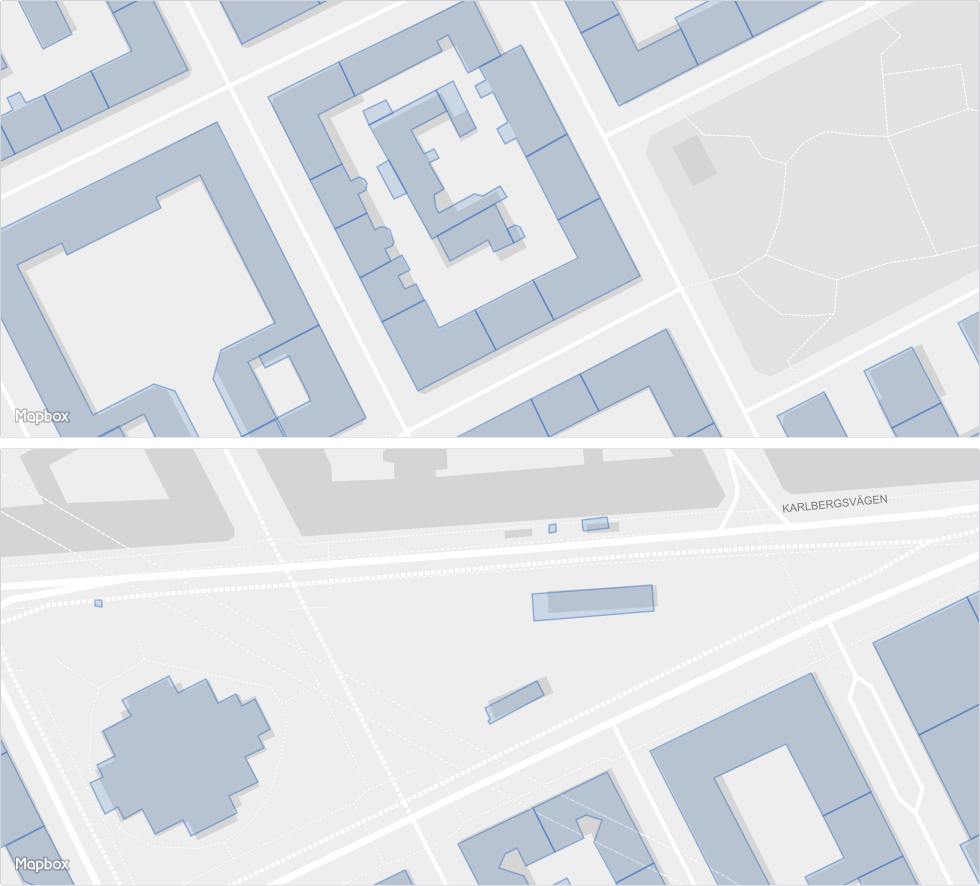
\includegraphics[width=\textwidth,height=0.5\textheight,keepaspectratio]{img_map_compare}
    \caption{Example segments of the Stockholm metropolitan area with unsystematic errors in precision. The SLU building dataset (blue) in superimposed on the OSM dataset (dark gray). The top picture is centered on a city block which shows a semantic mismatching between the two datasets. The whole block consists of only two buildings in the OSM dataset, but is divided into 15 smaller building lots in the SLU dataset. The bottom picture shows 4 smaller buildings whose the positional accuracy is low, due to the buildings being incorrectly scaled, skewed and rotated.}
    \label{fig:osm-slu-map}
\end{figure}

\subsection{Other accuracy criteria}

Let us briefly go over all of van Oorts accuracy criteria that will not be assessed through this study.
Let us see how they could be obtained and assessed for both the OSM and SLU maps, staring with the data lineage.
The lineage aspect of the OSM data is available through the OSM History Viewer, an online debugging tool that lets anyone freely view the change history of individual fetures in a commit history-like fashion.
There is an option for editors to include a personal note with their changesets to include additional details or motivate why a change was made, but there is no guaratee that the data includes any information on the aquisition method used \footnote{OSM History Viewer - OpenStreetMap Wiki. Accessed 20-03-2020. https://wiki.openstreetmap.org/wiki/OSM\_History\_Viewer}
The history aspect of the SLU dataset is not freely available online, but the acquistion method is included in the file metadata on a per-object basis.
Lantmäteriet uses internal codes to specifify the acquistion method, and these codes can be referred to in the product description the accompanies the map files.
As the scope of this project is limited to making a broad comparison of the positional accuracy of the two datasets, only the required positional accuracy as described by the SLU product description will be used.

The attribute accuracy measure is interesting, as both maps use encoded metadata on a per feature basis, the attribute accuracy of the two datasets could be assessed by doing a simple feature comparison and creating a translation table between the two attribute maps.
To the knowledge of the author, this has never been done with specifically these two datasets, at the time of writing.

The temporal accuracy will not be assessed as this projects focuses on comparing a single snapshot of the two datasets at the same point in time, and finally the logical accuracy will not be assessed because the underlying logical relations between features in both maps serve no purpose to this project.

\chapter{Background}

\section{Background of 3D city reproduction}

The project falls within the broader topic of geodata extraction and modelling, primarily of roads and building parcels.
Geodata modeling is at the foundation of procedural modelling of real-world cities, since any application which models cities based on geodata will need a robust method of aqquiring and laying out road and building data without compromising the data's integrity. \textbf{(Müller et al, 2006)}

Procedural modeling of road networks is of interest to the fields of urban planning and urban architecture. In recent years there has been an advent of interactive tools that aid urban planners in placing or generating features of an urban plan, particularly roads and road networks. Procedural and AI solutions that aid the arcitect in a form of human-machine symbiosis.

Procedural city-generation models combine architectural elemets, such as streets, lots, buildings, building facades.
Urban design practises with conventional two-dimenstional deliverables range from delivering neighbourhood designs, urban zoning and building plans, to writing design codes and building ordinances.
The last decade has seen multiple startups in the area of software that aid urban arcitecture. The software uses procedural models to render a city grid based on real-world locations, or generate new user-specified parameters, and allow for varying degrees of manual editing on grid, road, neighbourhood, city block or individual feature level.
Some of the most prominent examples are ArcGIS Pro (made by Esri), CityEngine (made by the startup Procedural, bought by ESRI) and Urban Canvas (made by the startup Synthicity, bought by Autodesk, now defunct).

But such tools are as of today not commonly applied in urbanist practises, due to failures in reflecting the unique workspace of arcitects and their design needs. Urban arcitecture is a social factors, stakeholders. Each arcitect is an actor in a continously developing environment, and affecting that environment in a complex manner through their action \textbf{(Stojanovski et al, 2020)}.

In recent years, there have been an advent of tools that extract geodata from OSM and generate 3D representations of real world locations by placing terrain, buildings, roads and other features.
However, freely available such tools seldom include smaller roads and pedestrian footpaths such as walkways, sidewalks or trails.

Additionally, the topic is of interest for 3D content creators in for example the fields of video game design or 3D animation. A trend in these fields is using methods of procedural modeling to create large amounts of 3D content quickly and efficiently, while requiring as little hand modeling as possible. Studios who create large worlds are often interested in solutions that generate large road networks without any hand modeling. \textbf{(Parish and Müller, 2001)}

\section{Related work}
When assessing the completeness of geodata, a very common scale is Van Oorts criteria for evaluating the quality of geographical information, which at the time of publication received attention from surveyors and cartographers.
\textbf{(Van Oort, 2006)} Since then a number of publications have examined slices of geodata from van Oort's criteria.
In 2008, \textbf{(Haklay, 2010)} conducted such a study to estimate of the quality of OSM positional geodata in London and England.
Since the OSM project started in London it was thought that OSM data in the London metropolitan area would be representative of the highest quality data available, and therefore a good indicator for the whole global OSM dataset.
The study was conducted by comparing OSM data to Ordnance Survey datasets.
The study showed that the OSM dataset had a rough positional accuracy of 6 meters from the reference dataset.
However, at the time of the study, the OSM project had captured roughly 29\% of the area of England, meaning that the data completeness was fairly low.

The next notable study to assess the quality of OSM data was published by \textbf{(Kunze, 2012)}.
The study applied different methods to assess the completeness of OSM data in two federal states in Germany, mainly by analysing the area difference between the OSM dataset and an administrative dataset.
Finally, a notable study in 2013-2014, conducted by researchers from various universities in Norway and Germany \textbf{(Fan et al, 2014)}, examined the quality and accuracy in building footprint data of the Munich area, at a time and place where the completeness of the OSM dataset was significantly higher (the results of their study showed that the OSM had captured close to 100\% of all building footprints).
At the time Munich was one of the most developed cities in OSM.
Their study included an insight in the geometrical calculations neccessary to match features and points between two datasets, and how to reliably calculate the metrics needed for the most important and assessible of van Oorts criteria.
Their study revealed that although the feature completeness of OSM was high, some architectural details were missing.
The results reveal that the positional accuracy of OSM data at the time was about 4 meters.

\chapter{Implementation}

\section{Geodata precision study}

\subsection{Assesment of dataset completeness}

\textbf{(Fan et al, 2014)} used the fraction of the total building area in their reference dataset and the OSM dataset to assess the completeness of OSM data.
The motivation for this is to eliminate semantic differences between both datasets.
A very common example of a semantic error when comparing geographic data is that a large building in one dataset may be segmented into several smaller ones in the other, that is to say a building in one set is represented as an aggreation of mutliple buildings in the other set.
This makes a complete one-to-one object mapping impossible.
Rather, buildings have to be identified as 1:1 (one to one), 1:n (one to many) or 1:0 (one to none) cases, depending on if a building is fully represented in the other dataset, represented as an aggregation of smaller plots, or not found at all.
Figure \ref{fig:building-match-types} shows examples of two buildings that were found in the OSM and SLU datasets as 1:1 and 1:n matches respectively.

Since it is impossible to find a one-to-one feature map for building footprints, using building area as an estimator for completeness is much better than i.e. using the number of buildings or other objects in each dataset.
This project will use the building area in the OSM dataset versus that of the SLU dataset to determine the completeness of OSM building data in the Stockholm area, which will then be used as an argument for how accurate the building correspondence and point proximity measures can be.

\begin{figure}[H]
    \centering
    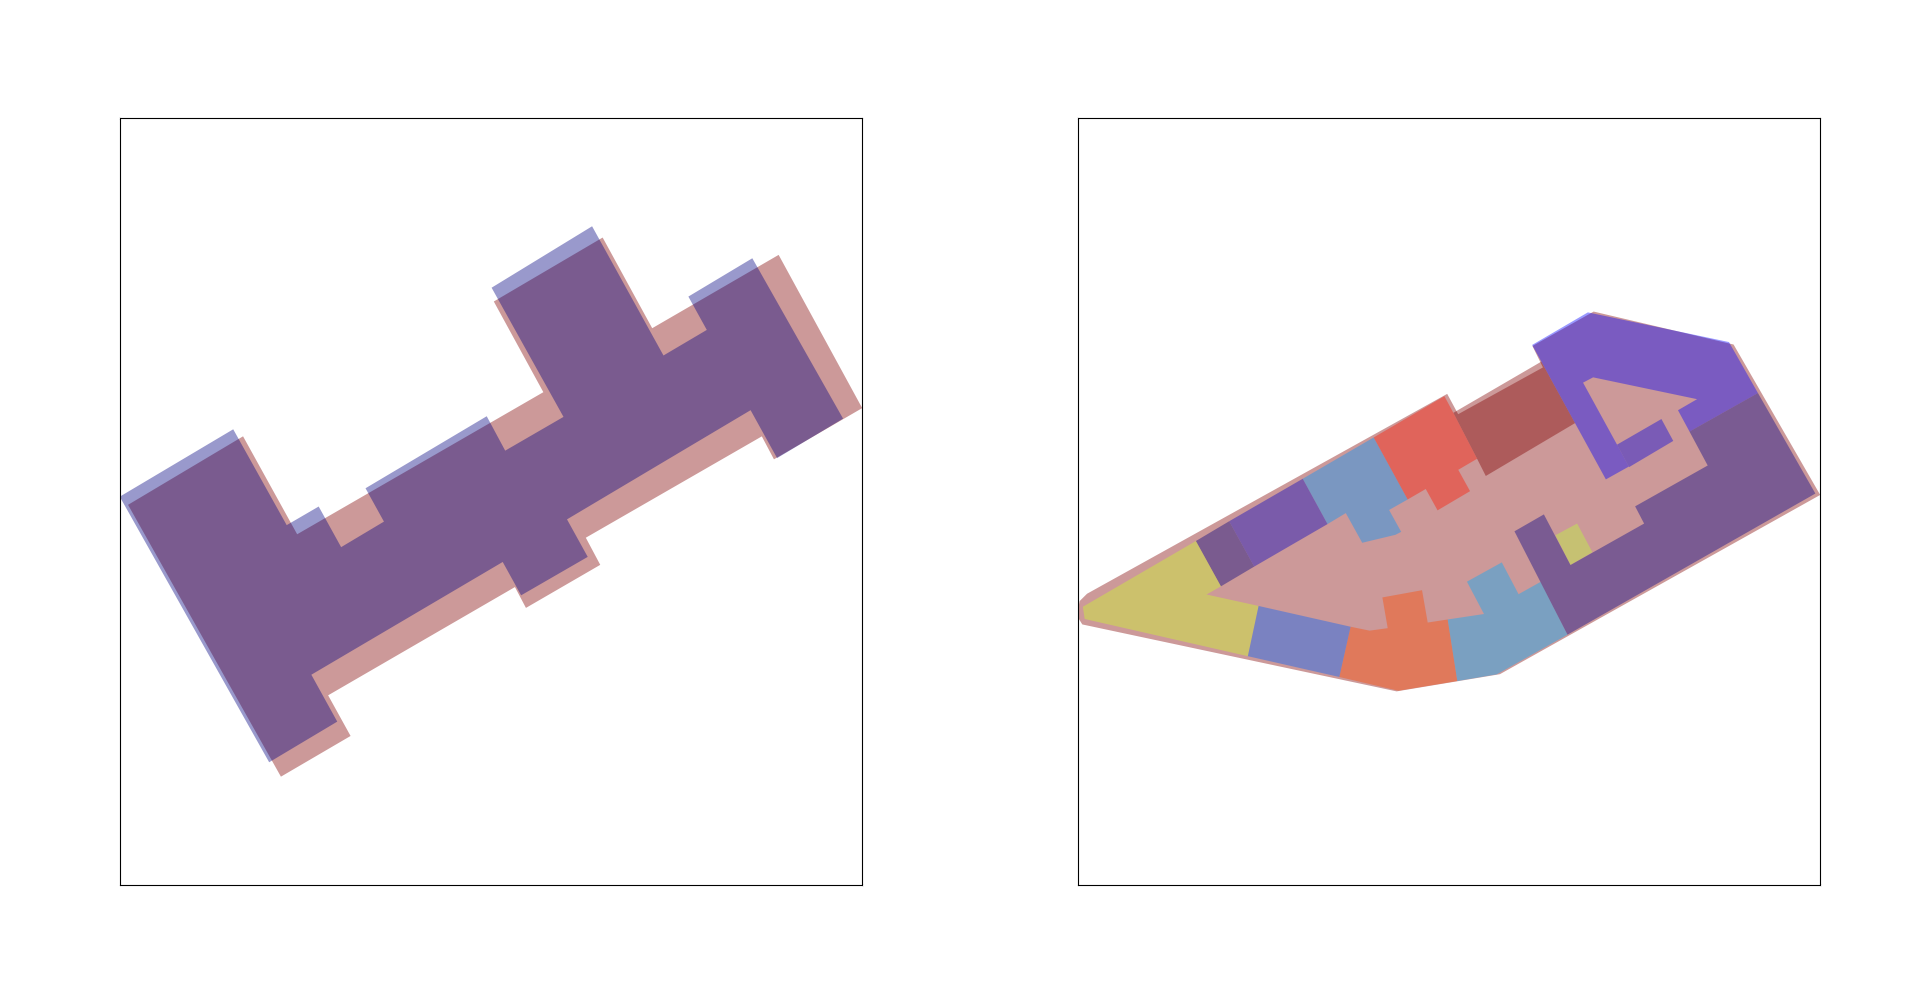
\includegraphics[width=\textwidth,height=0.5\textheight,keepaspectratio]{img_building_match}
    \caption{Examples of a 1:1 building match (left), where the sought-after building was found both in the OSM (red) and SLU (blue) datasets, and of a 1:n building match (right), where the sought-after building was represented as one polygon in the OSM (red) dataset, but divided into many smaller lots in the SLU (multicolored) dataset.}
    \label{fig:building-match-types}
\end{figure}

\subsection{Correspondence by building area}

\textbf{(Fan et al, 2014)} further discussed how the relative overlap in building area can be used as an estimate of the building correspondence between datasets.
In this project, relative area overlap was used in order to pair buildings from the two datasets together and create a feature map.
This can only be done in cases where there is not much displacement between OSM building footprints data and the reference data set.
Figure \ref{fig:osm-slu-map} under Section 5 shows a typical comparison between the OSM and SLU datasets.
By eyesight it was determined that the displacement of features is small.

The relative building overlap between the OSM and SLU datasets will be defined as folows, given the footprints of any building in the OSM set ($foot_{OSM}$) and the SLU set ($foot_{SLU}$):
\begin{center}
    $S_{RO}(foot_{OSM}, foot_{SLU}) = \frac{A_{Overlap}}{min(A_{foot_{OSM}}, A_{foot_{SLU}}))}$
\end{center}

The relative overlap may be used to determine building matching relations even when the semantic accuracy is low.
If a large building is represented by a single footprint in one dataset but by several smaller footprints in the other, \textbf{(Rutzinger, Rottensteiner and Pfeifer, 2009)} found that if $S_{RO}(foot_{A}, foot_{B}) < 30\%$ for two buildings $A$ and $B$ from different sets, then $A$ and $B$ are highly likely to be separate, neighbouring buildings and not in fact identical.
Therefore it will here be assumed that two buildings are matching candidates if their relative area overlap is greater than 30\%.
If a one-to-many object matching is found, the compound perimeter of the footprints in the many-set will be used when calculating the shape accuracy and finding closest vertices between the polygons.

When calculating the area overlap, it was utilized the fact that multipolygons in geojson are represented with the main, bounding polygon first.
Any subsequent polygons always represent cutouts or crop-outs in the footprint.
When calculating the area of a multipolygon building, the area of the first polygon was therefore taken and subtracted with those of the subsequent polygons.

\subsection{Shape accuracy definition}

The building footprint correspondence will be evaluated using a similarity function that depends on the difference between the turning funcitons of matching building footprints in both datasets.
The turning function was first defined by \textbf{(Arkin et al, 1991)}, as a method for measuring the similarity of two polygons.
The Turning function $T_c(l)$ measures the cumulative angle of the polygon's counter-clockwise tangent, as a function of the cumulative normalized length l.
This project uses the turning function as it is defined by \textbf{(Fan et al, 2014)}.
See figure \ref{fig:turning-function} for a side-by-side comparison of a polygon and its turning function.
For a polygon with vertices ${v_1 ... v_n}$ and line segments ${e_1 ... e_n}$ It is defined as follows.
Fix a starting vertex $v_1$.
The tangent angle at $v_1$ is $\theta_{n,1}$. This is the angle between the neighbouring line segments $e_n$ and $e_1$.
For any $i$ such that $i>1$ and $n<i$, the tangent angle at $v_i$ is recursively defined as:
\begin{center}
    $\theta_{i, i-1} = \theta_{n,1} + \sum^{i}_{k=1} \theta_{k, k-1}$
\end{center}
The turning function has some nice geometric properties, in that it is invariant to both rotation and scaling of the polygon. The function contains no information of the orientation of the polygon, only of the relative angle between successive line segments, thus it does not change under roation. It also measures only the normalized cumulative length, which does not change under scaling.
The similarity of two polygons A and B in terms of their turning function is defined as their distance of their cumulative turning functions:
\begin{center}
    $S_{T}(A, B) = 1 - (\int^{1}_{0} T_{C,A}(l) - T_{C,B}(l) dl)^{1/2}$.
\end{center}
The value range will be $(0 < S_{T} < 1)$, where $S_{T}(A,B) = 1$ if the polygons are identical. 
See figure \ref{fig:turning-function-compare} for a side-by-side comparison of two similar polygons and their turning functions.

\begin{figure}[H]
    \centering
    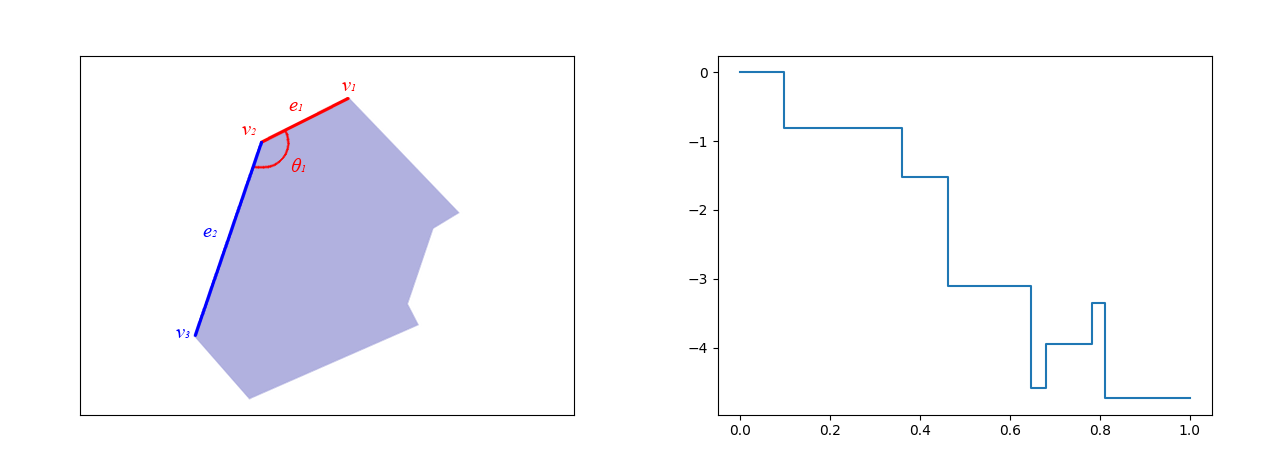
\includegraphics[width=\textwidth,height=0.5\textheight,keepaspectratio]{img_turn_function}
    \caption{An example of the turning function of a polygon. The edges, vertices and angle of the initial step of the turning funciton are marked.}
    \label{fig:turning-function}
\end{figure}

\begin{figure}[H]
    \centering
    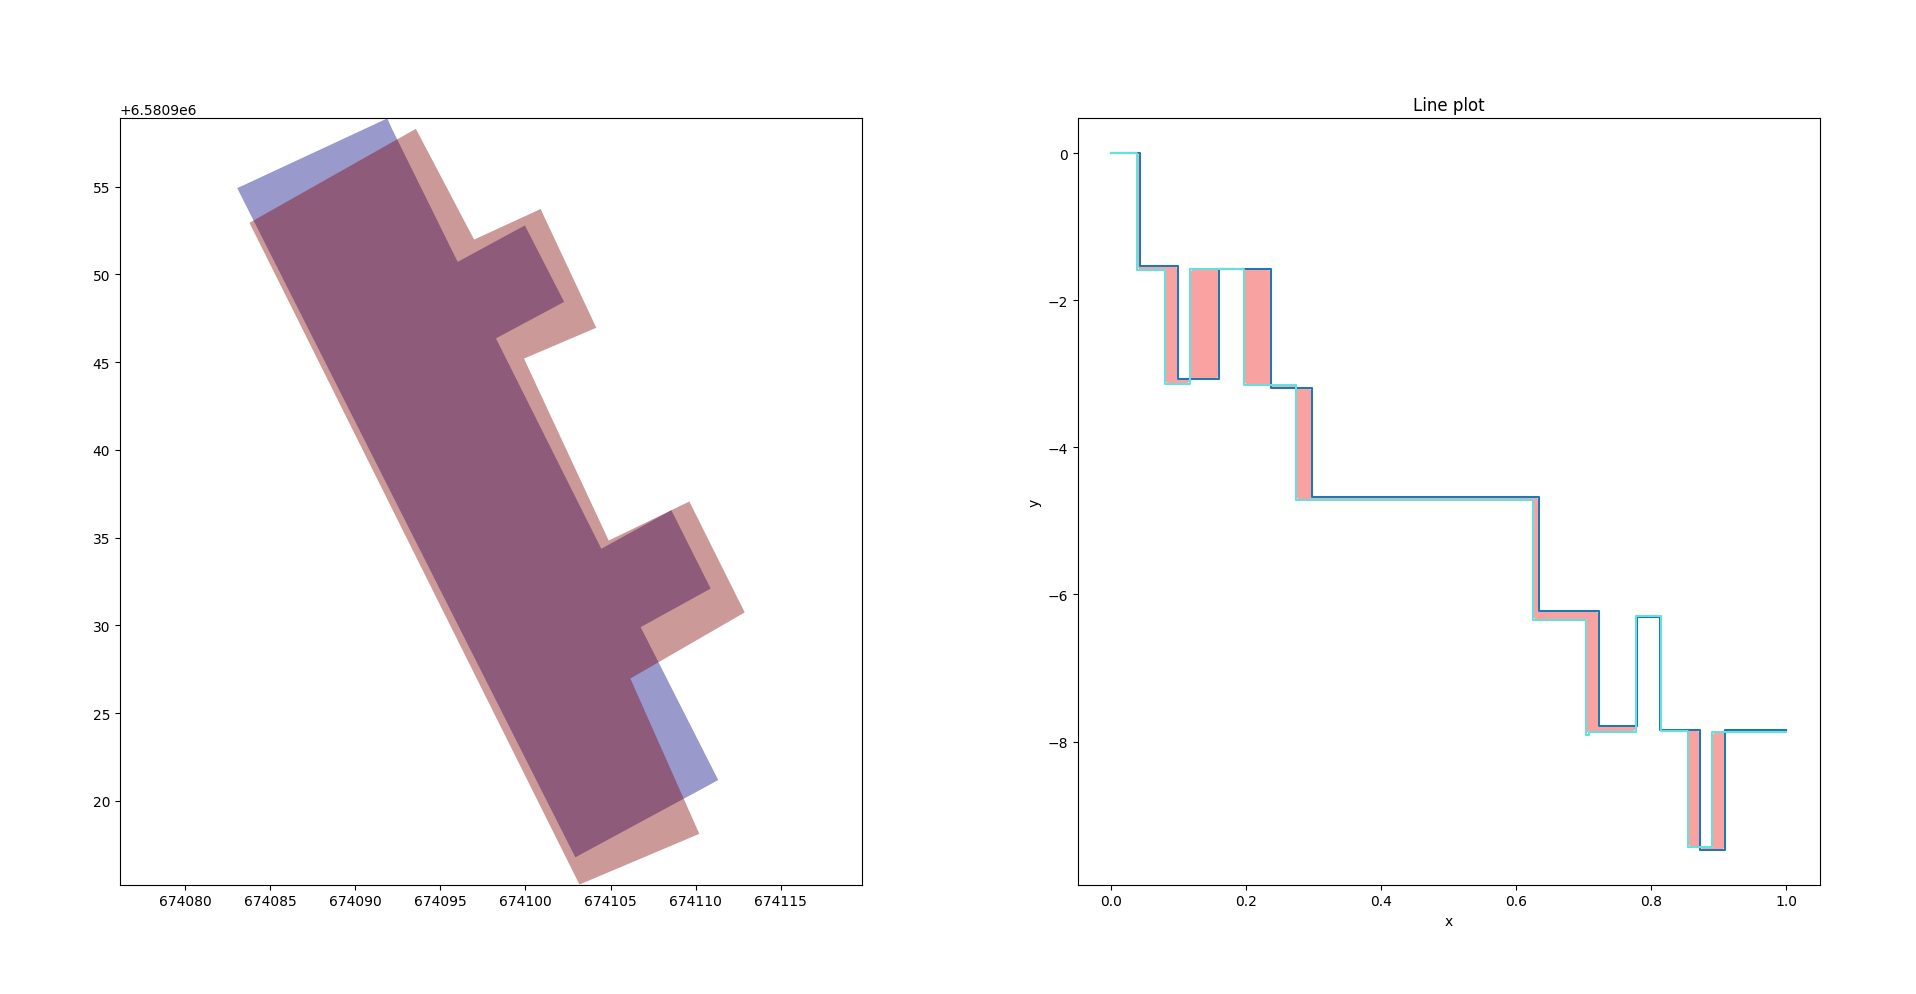
\includegraphics[width=\textwidth,height=0.5\textheight,keepaspectratio]{img_turn_function_diff_filled}
    \caption{An example of the turning functions of two corresponding buildings from the OSM and SLU datasets, with the area between them highlighted.}
    \label{fig:turning-function-compare}
\end{figure}

\subsection{Closest point and point proximity}

The final problem is that even when building polygons have been matched between the two datasets, they may not have one-to-one vertex relationship.
Footprints from different datasets may be formed at a different level of detail.
Problems that arise are e.g. that the vertex counts are dissimilar, or that vertex clusters may be found at different parts of the polygon in the two datasets.
To avoid this effect, key points are extracted using the Douglas-Peucker algorithm \textbf{(Douglas and Peucker, 1973)}, to create a simplifed footprint with less points that still retain information about the rough features of the detailed footprint.
The idea behind Douglas-Peucker is to recursively divide a polyline.
It initially marks only the start and end points $(v_0, v_n)$ to be kept, and finds the point $v_i$ in between whose distance is the greatest to the line segment between $v_0$ and $v_n$.
It then recursively refines the line segments $(v_0, v_i)$ and $(v_i, v_n)$, and proceeds to do so until a line segment $(v_j, v_k)$ is found, where every point in between $v_j$ and $v_k$ have a distance to the line segment $(v_j, v_k)$ that is smaller than some resolution $\epsilon$.
Then $v_j$ are added to the simplified polyline, and all nodes in between them are discarded.
See Algorithm 1 for a detailed view.
In either case The Oriented Minimum Bounding Rectangle (OMBR) is calculated for the two polygons.
Finally the OMBR for the OSM building footprint is shifted so that its centroid aligns with the centroid of the OMBR of the SLU building footprint.
Any edges in the simplified footprints that coinside with the OMBR from the same dataset are extracted, and the corresponding points in the original footprints will be matched with each other.
See figure \ref{fig:vertex-match-algo} for an illustration of the algorithm that detects matching vertices between two similar polygons.

\begin{figure}[H]
    \centering
    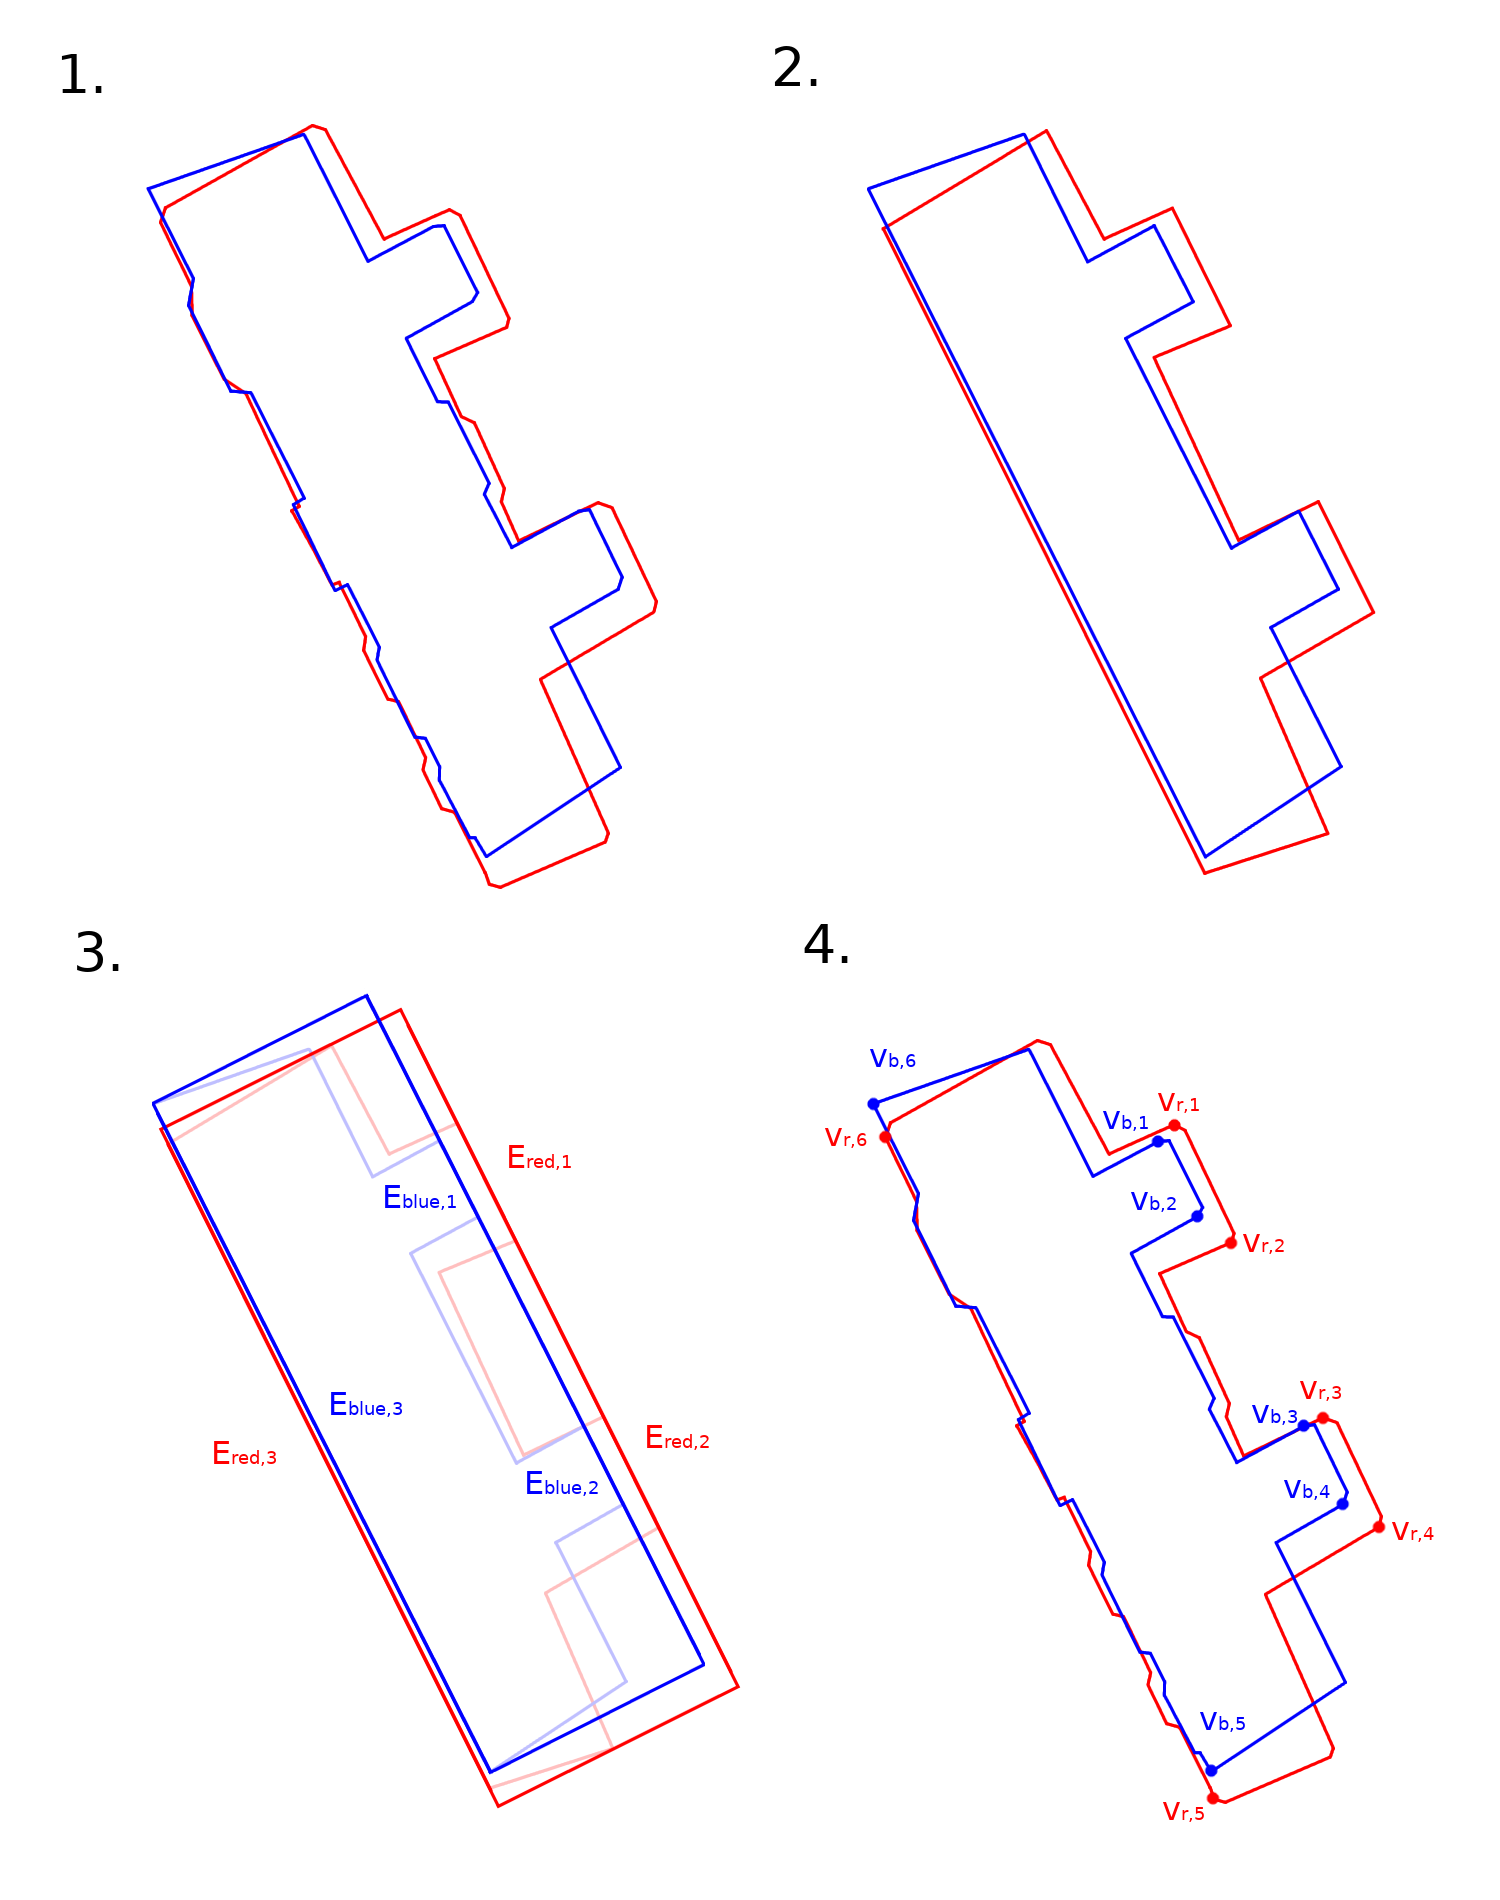
\includegraphics[width=\textwidth,height=0.5\textheight,keepaspectratio]{img_vertex_match_algo}
    \caption{An illustration of the matching vertices detection algorithm. Starting from two highly similar polygons, the first step is to obtain both the Douglas-Peucker reduced polygons. The next step is to obtain the OMBRs of the reduced polygons, and for both polygons find the edges that coinside with the edges of the OMBRs. These edges are corresponding, and thus their end vertices form a matching vertex map between the original polygons.}
    \label{fig:vertex-match-algo}
\end{figure}

\begin{algorithm}[H]
\SetAlgoLined
\KwResult{Write here the result }
    \textbf{Input:} PointList\\
    // Find the point with the maximum distance\\
    $d_{max}$ = 0\;
    $index$ = 0\;
    $end$ = length(PointList)\;
    
    \For{$i$=2 to ($end$-1)}{
        $d$ = perpendicularDistance(PointList[$i$], Line(PointList[1], PointList[$end$]))\;
        \If{$d$ $>$ $d_{max}$} {
            $index$ = $i$\;
            $d_{max}$ = $d$\;
        }
    }

    ResultList = []\;
    
    // If max distance is greater than epsilon, recursively simplify\\
    \eIf{$d_{max}$ $>$ $\epsilon$} {
        // Recursive call\\
        recResults1[] = Douglas-Peucker(PointList[1...$index$], $\epsilon$)\;
        recResults2[] = Douglas-Peucker(PointList[$index$...$end$], $\epsilon$)\;

        // Build the result list\\
        ResultList[] = {recResults1[1...length(recResults1) - 1], recResults2[1...length(recResults2)]}\;
    }{
        ResultList[] = {PointList[1], PointList[$end$]}\;
    }
    \Return{ResultList[]}\;

    \caption{Douglas-Peucker}
\end{algorithm}

Finally, when two building footprints and their vertices have been mapped, we will use the offset of matching vertices as a measure of positional error. The average and variance in vertex spread will be calculated and used to make an assessment of the geometric precision of the OSM dataset, and this precision will further be used to form an upper boundary on geometrical corrections that can be made to the map once it has been imported into the application.

\section{Collision study}

\subsection{Road widths and properties}

The maximum distance between two features was set to 1 times the positional accuracy, since then there will always be ample room to make changes to any features that would collide with the newly moved nodes, and thus we do not need to worry about feature collisions propagating.
In this implementation, roads of different types were allowed to merge into one another to form common intersections.
To facilitate this, it was neccessary to work with a path-by-path representation of the point data.
When two path share a node with common coordinates, they form an intersection which can be of multiple different types.

See the footnote for the publication that the default minimum widths were obtained from. \footnote{Vägars och gators utformning - Trafikverket. Publikation 2020:029. https://trafikverket.ineko.se/Files/sv-SE/71830/\\Ineko.Product.RelatedFiles/2020\_029\_vagar\_och\_gators\_utformning\_krav.pdf}
The standard recommended minimum width for a two-lane road in Sweden is 6.5 meters.

Subsequent visual measurements of a few key locations in the Stockholm area revealed the following minimum way widths:
Table \ref{table:road-widths} shows the minimum and maximum road widths that were found during these measurements, and that will be used in the collision study.

\begin{table}[H]
    \begin{tabular}{lllll}
                      & Footpath & Residential & Secondary & Primary \\
        Minimum width & 2.0 m    & 6.0 m       & 6.5 m     & 8.0 m   \\
        Maximum width & 5.0 m    & 9.0 m       & 10.0 m    & 16.0 m
    \end{tabular}
    \captionof{table}{Standard road widths used for the collision study}
    \label{table:road-widths}
\end{table}

\subsection{Feature Overlap algorithm}

The algorithm for determining feature overlap will calculate how many features and how many of their edges are intersecting with some other feature or edge.
It will also calculate the total length of all edge which are overlapping with some other edge.

The algorithm begins by iterating over all road features.
Let $A$ be the current road feature.
Since only road collisions are of interests, all roads were added to a queue and gone over one by one.
The polyline of the current road feature is extracted.
Then, all other candidate features for collision are iterated over, and their boundary polygons (for buildings) or polylines (for roads) are extracted.
Let $B$ be the current feature, road or building, that is being compared to $A$.
The algorithm then iterates over each edge $e_a$ in the polyline of $A$, and each edge $e_b$ in the polyline or polygon of $B$.
The Projected Line Segment Distance algorithm (See section 4.2.3) is used to determine the shortest distance between $e_a$ and $e_b$, and the smallest distance between any combination of edges $e_a$ and $e_b$ is taken to be the shortest distance between features $A$ and $B$.
If this distance is smaller than the minimum width of $A$, then $A$ and $B$ are colliding.

To speed up the collision checking process, a geometric hashing solution was developed.
In this way, feature collision lookup could be made without comparing a feature to all other available features, but instead from a selection of the closest candidates.
The hash bucket size was 230 by 230 meters and a feature could be in multiple hash buckets.

Here a few special cases are noted:
\begin{enumerate}
    \item If two roads intersect even though they share a node, it is a natural connection in the road network and should not be counted as a problematic case of feature overlap.
    \item Collisions between tunnels or bridges and other roads were ignored since these are of different heights. Brdiges and tunnels were identified by looking at feature attributes in OSM.
    \item Any roads that were represented as polygons or multipolygons instead of ploylines were also excluded from the study. These are typically town squares or areas designated for walking.
\end{enumerate}

\subsection{Projected Line Segment Distance}

The Projected Line Segment Distance (PLSD) algorithm is an extented version of the Line Segment Distance (LSD) algorithm.
Whereas LSD simply measures the distance between the two absolute closest points on two line segments, PLSD will yield the distance of the shortest vector $v$ between line segments $e_a$ and $e_b$, with the condition that $v$ is perpendicular to the tangent of $e_a$.
In the Feature Overlap algorithm, using the same notation as in section 4.2.2, PLSD takes $e_a$ to be the current edge of road feature $A$, and $e_b$ to be the current edge of feature $B$ (road or building).
See Algorithms 2 and 3 together for a detailed view of the PLSD algorithm.

\begin{algorithm}[H]
\SetAlgoLined
\KwResult{A float representing the shortests distance between $A$ and $B$}
    \textbf{Input:} Line segment $A$: [$\vec{a_1}$, $\vec{a_2}$], Line segment $B$: [$\vec{b_1}$, $\vec{b_2}$]\\
    // First assume that the points of $A$ and $B$ are ordered so that $\vec{a_1}$ is closer to $\vec{b_1}$ than to $\vec{b_2}$.\\

    // Check if the line segments $A$ and $B$ intersect, if so, the distance between them is 0.\\
    $\vec{x_s}$ = lineLineIntersection($A$, $B$)\;
    \If{$\vec{x_s}$ is not None} {
        \Return{0}
    }

    // Get the line-line intersection between the lines spanned by $A$ and $B$. If an intersection exists, it must lie outside of both $A$ and $B$.\\
    $\vec{x}$ = lineLineIntersection($A$, $B$)\;


    // Now that we have the intersection point, call the helper method to infer the shortest distance between $A$ and $B$.\\
    \Return{PLSD-Helper($A$, $B$, $\vec{x}$)}\;

    \caption{Projected Line Segment Distance}
\end{algorithm}

.\\

\begin{algorithm}[H]
\SetAlgoLined
    \textbf{Input:} Line segments $A$, $B$, intersection point $\vec{x}$]\\
    // Case 1: No intersection. The lines are parallel.\\
    \If{$\vec{x}$ is None} {
        \Return{perpendicularLineDistance($A$, $B$)}\;
    }

    // Get the projections of $\vec{b_1}$ and $\vec{b_2}$ on the line spanned by $A$:\\
    $\vec{d_1}$ = linearProjection($\vec{b_1}$, $A$)\;
    $\vec{d_2}$ = linearProjection($\vec{b_2}$, $A$)\;

    // Case 2: The projection of $B$ onto $A$ is completely disjoint from $A$ with no common points. No perpendicular distance can be inferred.\\
    \If{$(\vec{d_1}-\vec{a_1}) \cdot (\vec{d_1}-\vec{a_2}) > 0$ or $(\vec{d_2}-\vec{a_1}) \cdot (\vec{d_2}-\vec{a_2}) > 0$} {
        \Return{None}\;
    }

    // Case 3: $\vec{x}$ lies between $\vec{a_1}$ and $\vec{a_2}$.\\
    \If{$(\vec{x}-\vec{a_1}) \cdot (\vec{a_2}-\vec{x}) > 0$} {
        // Project the endpoints of $B$ on $A$, to find out which endpoint is closer to the intersection\\
        $d_{pl1}$ = pointLineDistance($\vec{b_1}$, $A$)\;
        $d_{pl2}$ = pointLineDistance($\vec{b_2}$, $A$)\;
        \eIf{$d_{pl1} < d_{pl2}$} {
            \Return{$d_{pl1}$}\;
        } {
            \Return{$d_{pl2}$}\;
        }
    }

    \eIf{|$\vec{x}$-$\vec{a_1}$| < |$\vec{x}$-$\vec{a_2}$|} {
        // Case 4: $\vec{x}$ is to the left of $\vec{a_1}$\\
        $\vec{a}$ = $\vec{a_1}$\;
        $\vec{b}$ = $\vec{b_1}$\;
    } {
        // Case 5: $\vec{x}$ is to the right of $\vec{a_2}$\\
        $\vec{a}$ = $\vec{a_2}$\;
        $\vec{b}$ = $\vec{b_2}$\;
    }

    $\vec{p}$ = linearProjection($\vec{b}-\vec{x}$, $\vec{a}-\vec{x}$)\;
    \eIf{|$\vec{p}$| < |$\vec{a}$-$\vec{x}$|} {
        $\vec{k}$ = $\vec{d}$\;
    } {
        $\vec{k}$ = $\vec{a}-\vec{x}$\;
    }

    $\theta = \arccos{|\vec{d}|/|\vec{b}-\vec{x}|}$\;
    \Return{$\tan{\theta} \cdot |\vec{k}|$}\;

    \caption{PLSD-Helper}
\end{algorithm}

\section{The geodata used in this project}

For the purpose of this project, the OSM road dataset has been sampled around Stockholm metropolitan area.
To assess and correct path widths and path node locations, the OSM building footprint dataset areound the same area has also been used.
As a reference dataset, the property map from the Swedish National Land Survey was used in comparison with the OSM map.
The reference map is provided by the Swedish University of Agricultural Sciences (SLU), and will be referred to in this report as the SLU map or the SLU dataset.
The SLU map conatins only building and property footprints.
The exact map segments that were extracted were in both cases rectangular boundaries with the following coordinates in WGS84: (N: 59.42, E: 18.15, S: 59.23, W: 17.79).
Both datasets were collcted on March 18th, 2020.

\subsection{OSM data}

The OSM project is a wiki-like geodatabase based on Volunteered Geographical Information (VGI), meaning anyone can contribute by adding or editing features.
OSM road data and building footprints are commonly obtained by manually tracing features in commercially available satellite images.
Such images have a limit on their resolution which puts a theoretical limit on the accuracy of map features compared to their real-world equivalents (Haklay 2010).
Particularily the high resolution imagery from Bing in 2010 led to an increase in building information in OSM, and the positional error is largely due to the limited resolution in such satellite imagery. \textbf{(Fan et al, 2014)}.

\subsection{SLU data}

The SLU map is maintained by The Swedish National Land Survey (Swedish: Lantmäteriet).
The data is collected by geodetic professionals, by land surveying methods such as GPS or DGNSS positioning, or by reproduction of features from ortophoto or stereo mapping from 3D aerial images.
Building features in the SLU dataset have a position accuracy requirement of 2 meters.
The SLU map contains building features and property limits, but no road data.
The map is updated continously by Lantmäteriet, in conjoncture with the forming or reforming of property.
Whereas OSM is a free service, the SLU map is available to paying customers or for free to students and researchers. \footnote{Lantmäteriet. Produktbeskrivning: GSD-Fastighetskartan vektor - Lantmäteriet. Acessed 16-04-2020. https://www.lantmateriet.se/globalassets/kartor-och-geografisk-information/kartor/fastshmi.pdf}

\subsection{A word on coordinate systems}

The SLU dataset is delivered in the SWEREF 99 TM coordinate system.
SWEREF 99 TM is a projected coordinate system and there is no linear transformation to the WGS 48 system, which OSM uses. \footnote{Converting to WGS84 - OpenStreetMap Wiki. Accessed 13-03-2020. https://wiki.openstreetmap.org/wiki/Converting\_to\_WGS84}
The coordinate conversions for this paper were obtained using proj: a Linux commandline application for geospatial coordinate conversion.

\subsection{Specific geodata preprocessing}

Upon delivery of the OSM dataset, all features that intersect with the user-specified domain are included, with their full geometry.
The SLU map however, is delivered with building footprints cropped to exactly match the query coordinates, meaning that buildings at the edge of the user-specified domain can have cropped geometries.
Any building area outside of the query domain will be excluded.
Since the principles behind what features are delivered and how differ between the datasets, it is neccessary to crop both datasets to ensure that all buildings are complete and have matching candidates in the other set.
Any features that intersect the edge of the rectagular boundary, in both datasets, were therefore excluded from the study.

\chapter{Results and metrics}

\section{Road collision study}

For the primary collision study.
Table \ref{table:road-collision} shows the statistics of the collision study, and the number of roads, number of edges and total edge length that showed intersections with other features before road extrusion, by road category.
For footpaths in particular, it was shown that 12.05\% of all roads collide with some other feature after extrusion to the minimum width.
The same was shown to be true for 0.11\% of the road polyline edges and 0.09\% of the total road length.
Table \ref{table:road-collision-corrected} shows the remaining roads, edges and total edges length whose intersections with other features could not be resolved by geometrical translation of a distance smaller than the positional accuracy.
For footpaths this was shown to hold of 0.51\% of all roads, 
The number of road edges and percentage of the total road length that could not be corrected by geometric translation was significantly small.

\begin{table}[H]
    \begin{tabular}{lllll}
                                & Footpath      & Residential  & Secondary   & Primary     \\
        Features, total         & 26473         & 10523        & 3044        & 2756        \\
        Edges, total            & 6382579       & 6612383      & 968420      & 420810      \\
        Edge length, total      & 129984.79 km  & 186089.55 km & 29304.57 km & 16162.95 km \\
        Features, colliding     & 3189          & 1032         & 412         & 456         \\
        Edges, colliding        & 7330          & 2362         & 643         & 824         \\
        Edge length, colliding  & 110.67 km     & 66.18 km     & 9389.30 m   & 20.41 km    \\
        Features, percent       & 12.05 \%      & 9.81 \%      & 13.53 \%    & 16.55 \%    \\
        Edges, percent          & 0.11 \%       & 0.04 \%      & 0.07 \%     & 0.20 \%     \\
        Edge length, percent    & 0.09 \%       & 0.04 \%      & 0.03 \%     & 0.13 \%

    \end{tabular}
    \captionof{table}{The first result table of the collision study. This table shows the amount of features and edges, as well as the cumulative edge length, in total and which are intersecting with any other feature.}
    \label{table:road-collision}
\end{table}

\begin{table}[H]
    \begin{tabular}{lllll}
                                & Footpath      & Residential  & Secondary   & Primary     \\
        Features, colliding     & 134           & 336          & 246         & 277         \\
        Edges, colliding        & 157           & 530          & 306         & 407         \\
        Edge length, colliding  & 3248.73       & 6475.99 m    & 3840.00 m   & 8039.54 m   \\
        Features, percent       & 0.51 \%       & 3.19 \%      & 8.08 \%     & 10.51 \%    \\
        Edges, percent          & 0.00 \%       & 0.00 \%      & 0.03 \%     & 0.09 \%     \\
        Edge length, percent    & 0.00 \%       & 0.00 \%      & 0.01 \%     & 0.05 \%

    \end{tabular}
    \captionof{table}{The second result table of the collision study. This table shows the amount of features and edges, as well as the cumulative edge length, which can be corrected by simple geometric translation.}
    \label{table:road-collision-corrected}
\end{table}

\section{Positional accuracy study}

For the secondary study, the average positional accuracy per building was calculated to roughly 2.06 meters, and this will be taken as an estaimate of the positional accuracy of the OSM dataset.
Table \ref{table:positional-accuracy} shows the estimate in positional accuracy that was obtained from the study.
Figure \ref{fig:bar-plot-positional-accuracy} shows the positional accuracies measured per building as a frequency diagram.

\begin{table}[H]
    \begin{tabular}{lllll}
        $e_{average}$ & $e_{max}$ & $e_{min}$ & $e_{standard deviation}$ \\
        2.0579... & 9.9878... & 0.0 & 1.2464...
    \end{tabular}
    \captionof{table}{The estimated positional accuracy of the OSM dataset: average, max, min and standard deviation}
    \label{table:positional-accuracy}
\end{table}

\begin{figure}[H]
    \centering
    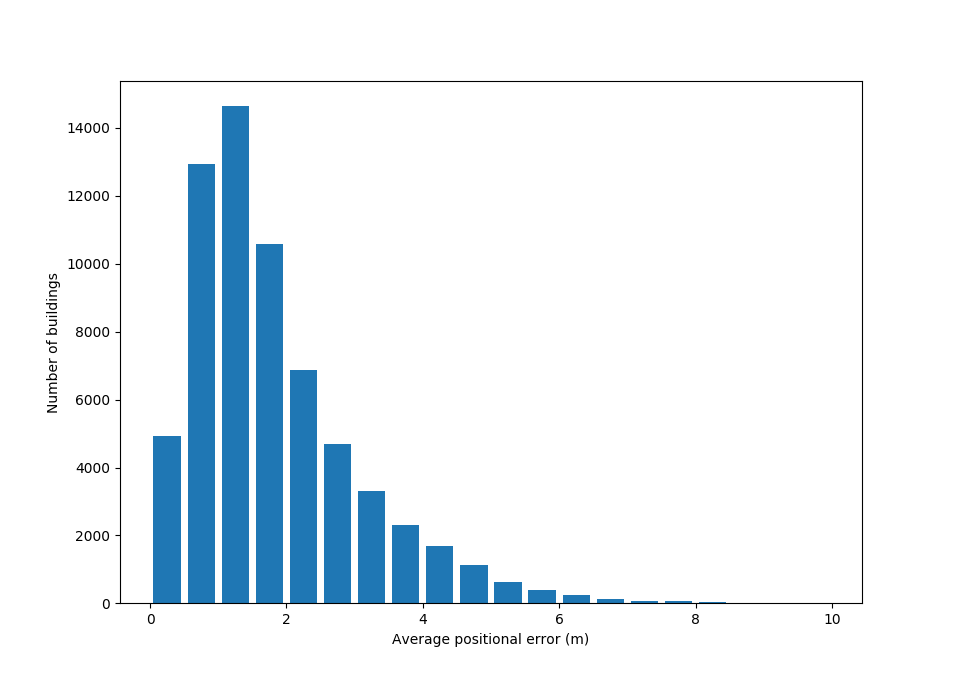
\includegraphics[width=\textwidth,height=0.5\textheight,keepaspectratio]{img_pos_error_plot}
    \caption{The average positional accuracies per building as a frequency diagram.}
    \label{fig:bar-plot-positional-accuracy}
\end{figure}

\section{Secondary metrics}

\subsection{Completeness by building area}

Table \ref{table:num-of-buildings} shows the building coverage of the OSM and SLU datasets in terms of the number of buildings and their total area.
Table \ref{table:num-of-buildings-percent} shows the building coverage of both datasets as perentages.
The area cover of the OSM dataset in relation to the SLU dataset was estimated to 98.18\%. This will be taken as an estimate of the completeness of the OSM dataset.

\begin{table}[H]
    \begin{tabular}{lllll}
        & Total number of buildings & Area cover \\
        OSM & 102755 & 33105023.32... $m^2$ \\
        SLU & 170783 & 33718628.97... $m^2$
    \end{tabular}
    \captionof{table}{Total number of buildings and their cumulative area}
    \label{table:num-of-buildings}
\end{table}

\begin{table}[H]
    \begin{tabular}{lllll}
        & Number of buildings (\%) & Area cover (\%) \\
        OSM & 60.17\% & 98.18\% \\
        SLU & 100.00\% & 100.00\%
    \end{tabular}
    \captionof{table}{Total number of buildings and cumulative area as percentages}
    \label{table:num-of-buildings-percent}
\end{table}

\subsection{Building matching statistics}

Table \ref{table:building-matching} shows how many of the OSM to SLU building matches were found in each category of 1:1, 1:n and 1:0 matches.

\begin{table}[H]
    \begin{tabular}{lllll}
        & 1:0 & 1:1 & 1:n & Total \\
        Match count & 9812   & 81722   & 11221   & 102755 \\
        Percent     & 9.55\% & 79.53\% & 10.92\% & 100\%
    \end{tabular}
    \captionof{table}{The number and percentages of matching buildings between both datasets, ordered by type of correlation (1:0, 1:1 or 1:n)}
    \label{table:building-matching}
\end{table}

\subsection{Shape accuracy statistics}

Figure \ref{fig:bar-plot-similarity} shows the shape similarity measured per building as a frequency diagram.

\begin{figure}[H]
    \centering
    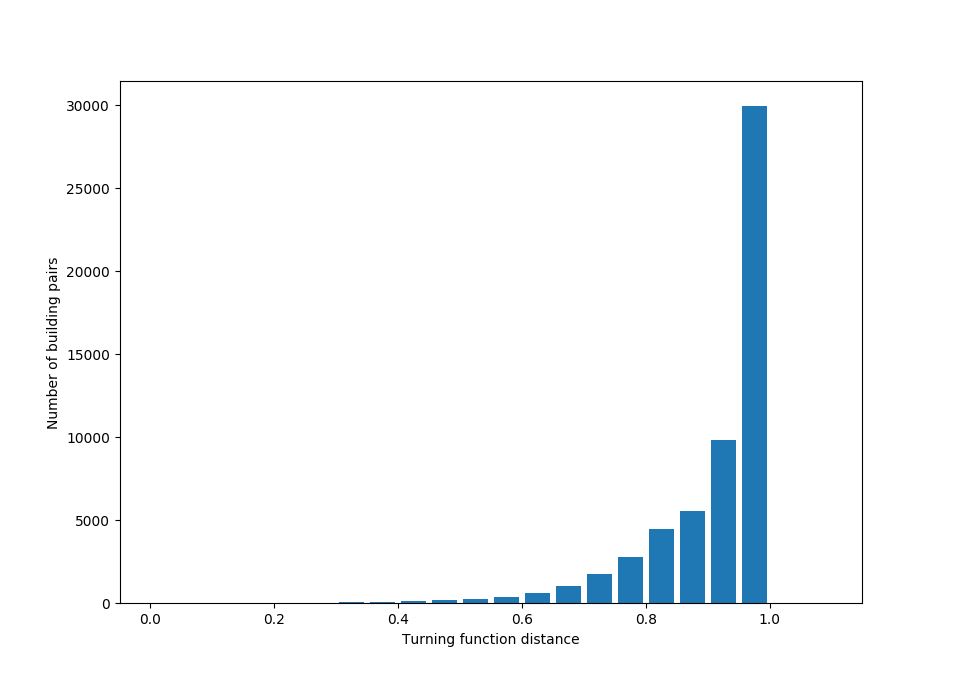
\includegraphics[width=\textwidth,height=0.5\textheight,keepaspectratio]{img_turning_function_plot}
    \caption{The shape similarities between 1:1 building pairs as a frequency diagram.}
    \label{fig:bar-plot-similarity}
\end{figure}

\chapter{Analysis}

\section{Quality of the OSM dataset}

The completeness analysis by building area shows that the OSM Stockholm dataset has high completeness in terms of both building area and counted features, in the same level as the study of Munich by \textbf{(Fan et al, 2014)}.
The difference in area cover can partially be explained by small utility buildings that are often not represented in the OSM dataset.
Particularily the residential areas in downtown, Stockholm, are characteristic in that each city block consists of a street front and an open, communal compound in the middle, inside of which there are usually a number of small utility buildings such as bicycle garages, toolsheds, refuse rooms and such.
See figure \ref{fig:osm-slu-map-utility-buildings} for an example of an area in stockholm with such characteristics.
These buildings are likely hard to make out and trace on publicly available satellite image data.
They are, according to \textbf{(Fan et al, 2014)} occluded by their surroundings due to shadows or forestry.
This appears to be a large consensus in the field.

The low semantic accuracy has made analysis hard.
The available SLU dataset from Lantmäteriet uses a plot-based subdivision of buildings, whereas OSM uses a subdivision that more closely resembles the actual building footprint as seen from above.
In many cases whole city blocks are represented as single buildings, which means that many less meaningful feature matches can be found.
As seen in table \ref{table:building-matching}, about 80\% of all OSM features were found to have a 1:1 mapping to the SLU dataset, but upon further visual comparison it can be seen that many of the 1:n matches are found in a very specified area, namely the residential areas in downtown, Stockholm.
This is problematic since this typical area with the same level of accessibility was likely measured with the same measuring technique, and the unsystematic positional error will likely be similar in these areas.
The question is wether it comforms well to the positional error in the rest of the dataset or not.
This analysis will not be carried out in this project, but could be a good subject for a future master's thesis project.

\begin{figure}[H]
    \centering
    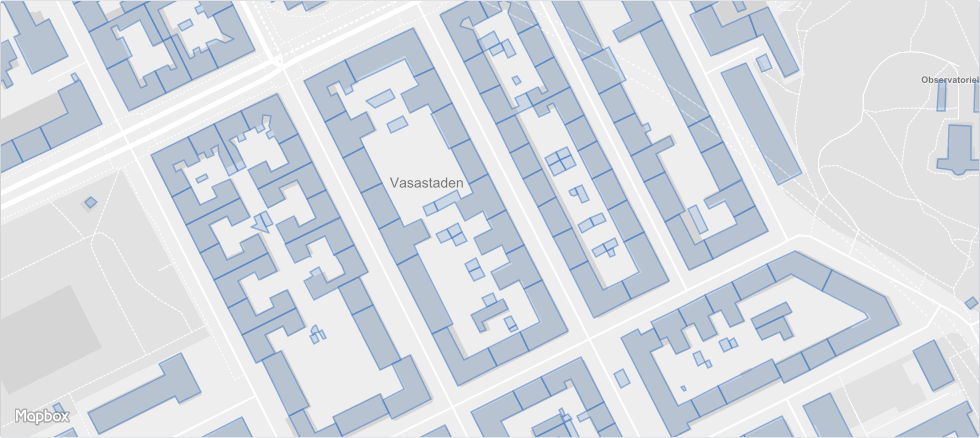
\includegraphics[width=\textwidth,height=0.5\textheight,keepaspectratio]{img_map_utility_buildings}
    \caption{A map segment which shows an area with many small utility buildings that are represented in the SLU dataset but not in the OSM dataset.}
    \label{fig:osm-slu-map-utility-buildings}
\end{figure}

% Report, restructuring
% TODO: Summarize Analysis in Conclusions
% TODO: Conclusions headlines
% TODO: Overview at the beginning of each chapter

% After next meeting with Chris
% TODO: Spell check
% TODO: Go over report one final time
% TODO: Swedish abstract

\section{Collision study}

The immediate conclusion of this study is that, in terms of feature collision, footpaths were not significantly worse than other road categories.
As a result, it can promptly be assumed that city modelling services which already utilize OSM car road data could also use OSM footpath data without a drastic increase in feature collision.
The biggest reason for this is thought to be that footpaths in their nature are narrow.
So narrow in fact that they can be displaced by more than half of their full width (minimum 1 meter) before the limit of half the positional accuracy (1.025 meters) is reached.

Looking closer at the individual collision cases, the next conclusion is that most often it is actually a small part of a road that is colliding, and will need correction.
We make an exemplifying calculation to support this claim.
Looking in tables \ref{table:road-collision} and \ref{table:road-collision-corrected}, we note that before road extrusion, 3189 features and 7330 of their edges are intersecting some other feature.
This means that for each colliding road, on average 2.3 of its edges will be intersecting some other feature, thus bearing responsibility for the collision.
In total there are 26473 feautures and 6382579 edges, meaning that each road feature is on average contructed out of 241 edges.
Thus the percentage of edges colliding per road is on average roughly 0.95\%.
A similar calculation for the number of features that could not be corrected by translation yields that the number of colliding edges per feature is on average 1.2, and that the percentage of colliding edges per feature is 0.49\%.
Visual inspection of the cases where roads collide with other features has supported this.

After visual inspection of the cases where features collide, it was determined that all collision occurences can be almost exclusively classified into one of five categories.
These categories are explained in the list below, and each case is exemplified in figure \ref{fig:collision-cases}.
All these cases will create issues when generating the 3D mesh representation of the city.

\begin{enumerate}
\item Case 1: A building lies in paralel with a road, and the distance between the two is smaller than the minimum width of the road.
\item Case 2: A road shares a node with a building.
\item Case 3: A road is intersecting with certain building features.
\item Case 4: Two roads have a minimum distance that is smaller than the sum of the minimum widths of both roads. 
\item Case 5: Two roads share a node, and a subsequent node in one road lies within the minimum width of the other road.
\end{enumerate}

\begin{figure}[H]
    \centering
    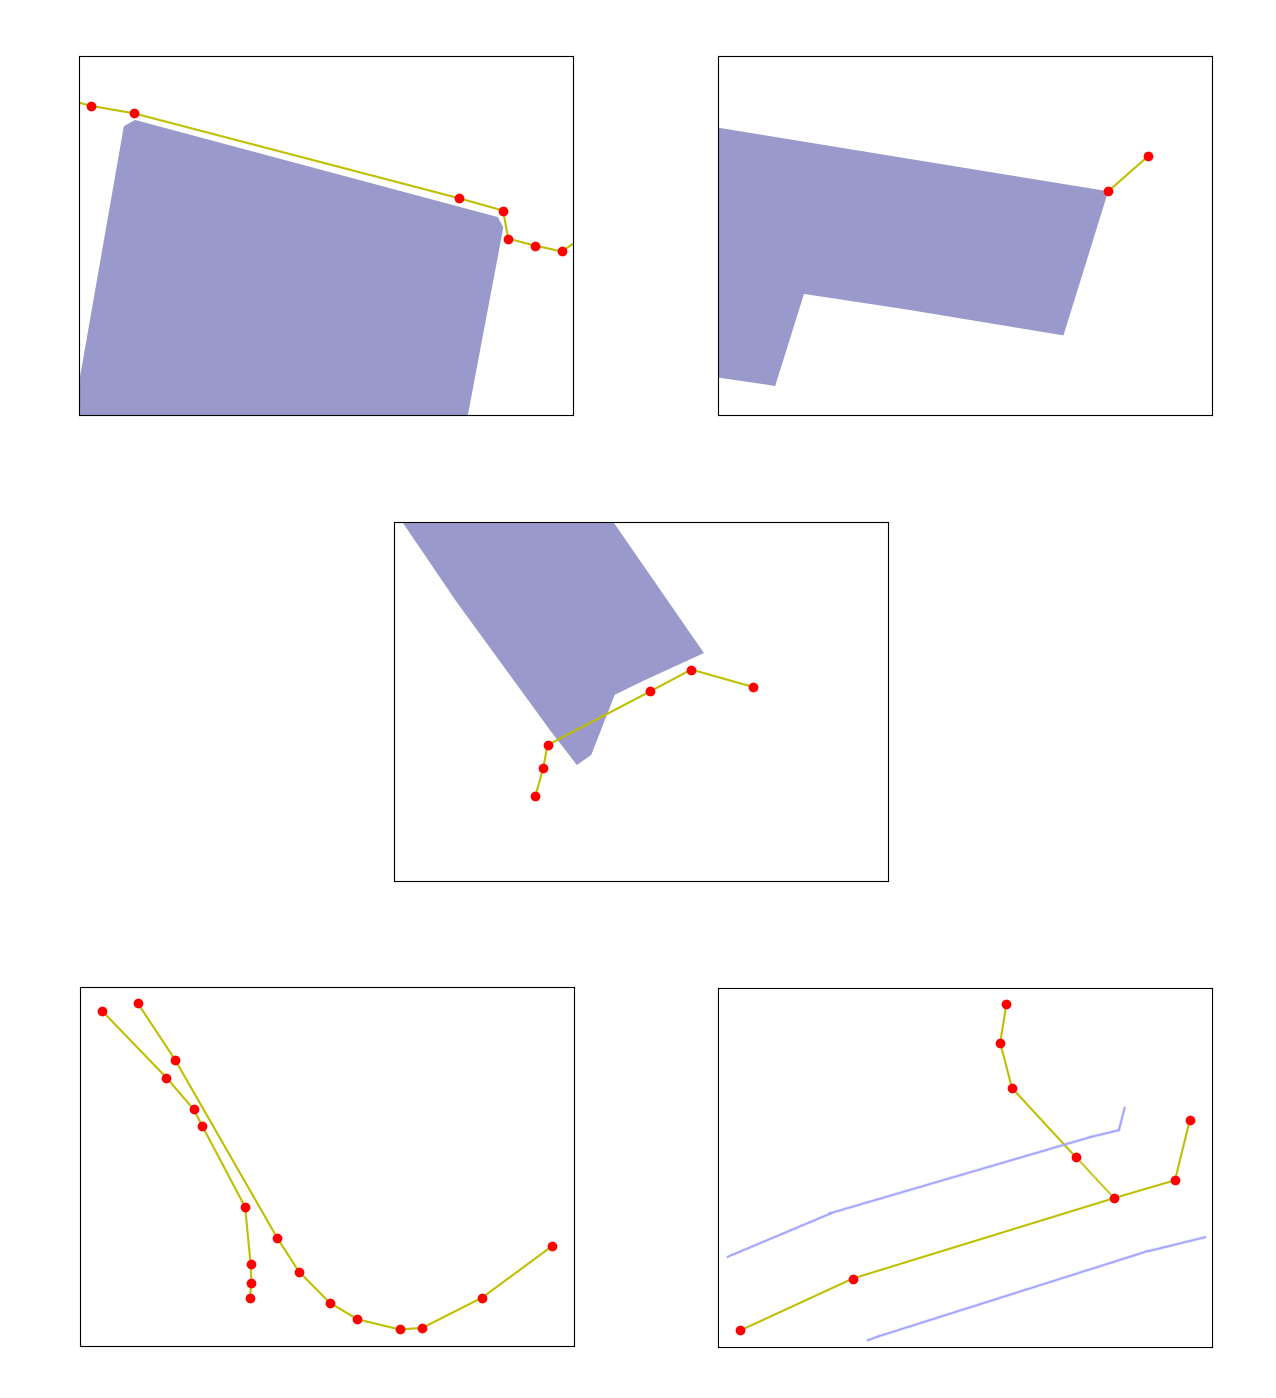
\includegraphics[width=\textwidth,height=0.5\textheight,keepaspectratio]{img_feature_overlap_cases}
    \caption{The 5 identified cases over feature overlap. Top left: Case 1. Top right: Case 2. Middle: Case 3. Bottom left: Case 4. Bottom right: Case 5.}
    \label{fig:collision-cases}
\end{figure}

\section{Suggested algorithms for collision correction}

All collision cases can be solved with relatively simply geometric algorithms. This section will present suggestions on algorithms that will resolve collisions by identifying individual colliding nodes and translating them, after which some degree of smoothing (such as linear interpolation) can be applied to preserve visual features. Cases 1 and 3-5 will be handled, while 2 will be left since case 2 collisions do not inherently cause feature overlap when extruding a 3D road mesh from the way edges. Thus it will me up to the individual developer to decide what to do with Case 2 collisions.

\begin{enumerate}
\item Case 1 collisions can be solved by translating colliding way points away from the building, along the normal of the nearest surface. Smoothing can then be applied as seen fit.
\item Case 3 collisions can be solved by eliminating the building features that intersect with the way, and then applying the same algorithm as in case 1.
\item Case 4 collisions can be solved by calculating the average normal over all colliding edges for both roads, and translating colliding points along the normal, away from the other road. Smoothing can then be applied as seen fit.
\item Case 5 collisions can be solved simply by translating the colliding point along the tangent of the closest edge, and then applying smoothing as seen fit.
\end{enumerate}

\begin{figure}[H]
    \centering
    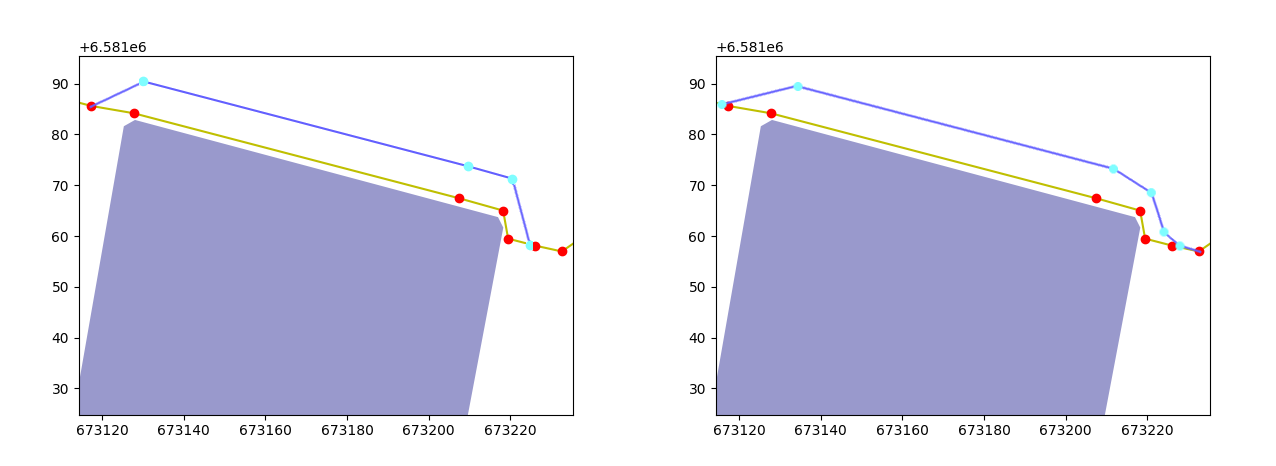
\includegraphics[width=\textwidth,height=0.5\textheight,keepaspectratio]{img_feature_overlap_fix_1}
    \label{fig:collision-case-1}
    \caption{Example of the solution algorithm for case 1 collision. The yellow line shows the original road placement. The blue line shows the updated road placement. The second picture illustrates how smoothing can be applied to the translated road if desired.}
\end{figure}

\begin{figure}[H]
    \centering
    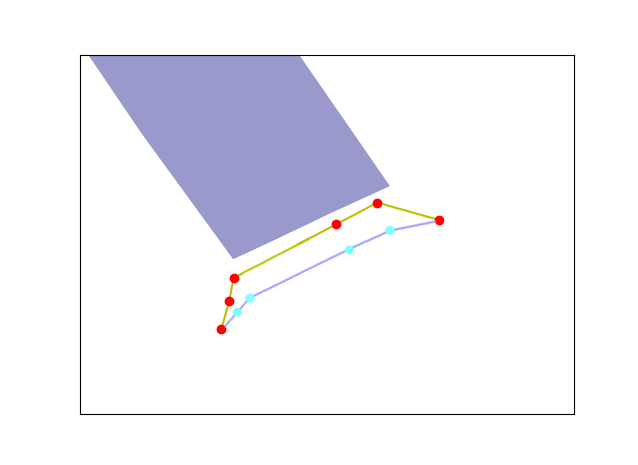
\includegraphics[width=\textwidth,height=0.5\textheight,keepaspectratio]{img_feature_overlap_fix_2}
    \label{fig:collision-case-3}
    \caption{Example of the solution algorithm for case 3 collision. The portruding building feature as seen in \ref{fig:collision-cases} has been eliminated. The yellow line shows the original road placement. The blue line shows the updated road placement.}
\end{figure}

\begin{figure}[H]
    \centering
    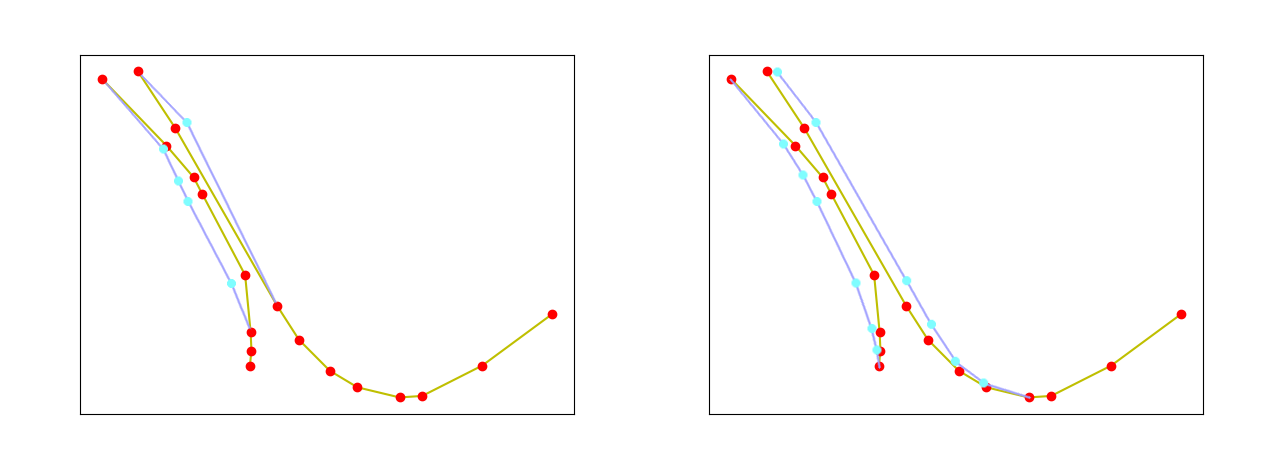
\includegraphics[width=\textwidth,height=0.5\textheight,keepaspectratio]{img_feature_overlap_fix_3}
    \caption{Example of the solution algorithm for case 4 collision. The yellow lines show the original road placements. The blue lines show the updated road placements. The second picture illustrates how smoothing can be applied to the translated road if desired.}
    \label{fig:collision-case-4}
\end{figure}

\begin{figure}[H]
    \centering
    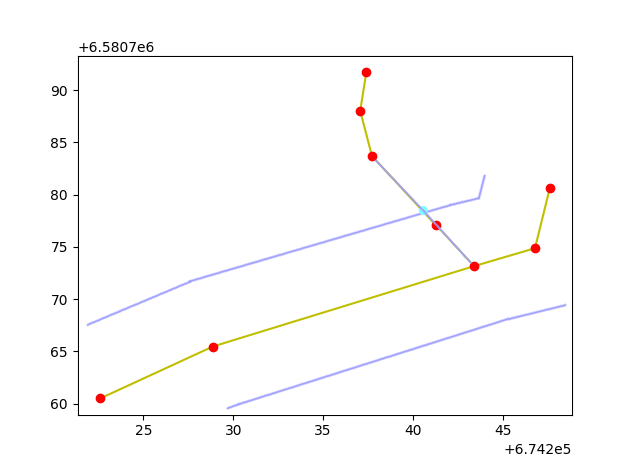
\includegraphics[width=\textwidth,height=0.5\textheight,keepaspectratio]{img_feature_overlap_fix_4}
    \caption{Example of the solution algorithm for case 5 collision. The yellow lines show the original road placements. The blue line segment with the cyan vertex shows the updated placement of the interesting vertex. The remaining blue lines show the boundaries of the original road.}
    \label{fig:collision-case-5}
\end{figure}

\chapter{Conclusions and future work}

\section{Data conclusions}

One could reasonably assume that Stockholm, being one of the more developed cities in one of the most technologically connected country in the world, would be fairly well mapped in OSM.
Let us take the positional accuracy of the Stockholm area, as obtained by this study, as reprentative of that of major cities in developed countries in the OSM dataset.
Then the positional accuracy has improved by roughly 3.5 meters since the study by \textbf{(Haklay, 2010)}, and by roughly 1.5 meters since the study by \textbf{(Fan et al, 2014)}.
This of course assumes that the SLU reference dataset is taken as absolute.

\section{Scientific field study}

We now have a firm idea of the technical feasibility of generating virtual cities from OpenStreetMap-data, including different types of road networks.
We have however yet to touch upon the importance for road network modelling in the broader context of 3D city reproduction.
Where exactly in the pipeline of reconstructing a virtual city does this happen, and what are the remaining challenges?
This will be the goal of this final scientific study: to place everything we have learnt so far in the broader context of GIS and city modeling, and the respective research fields.

As has been mentiond in the introduction to this report, procedural generaion of road networks is a basal requirement for quick and low-effort modeling virtual cities.
Since the road network ties together the city, and forms the grid that divides the lots, quarters and neighbourhoods, it make sense that we can only continue with the remaining challenges once we can a robust procedure for extracting road geodata and generating the 3D represention of it without compromising the data integrity. 
The same is true for building modelling.
It turns out that the same methods that have been used in this project to obtain and qualify road network data can be applied to building footprint data from OSM. \textbf{(Fan et al, 2014)}
And only when we have such a fundamental procedure for accuratly importing building footprints without compromising the data integritey, we can proceed with the remaining challenges in building modeling. \textbf{(Müller et al, 2006)}

Such challenges, which have not been mentioned up until this point, include infering or guessing building height, since OSM does not provide data about building elevation.
Occasinally buildings in OSM may be tagged, but the norm is that no elevation data is available.
There are however very sophisticated methods from guessing the building height after looking at reference datasets.
\textbf{(Biljecki, Ledoux and Stoter, 2017)} presented a method for inferring building height exclusively from the building footprint and surrounding footprints.
Surprisingly, their model was shown to be accurace within a meter on average.

Another challenge is that of including terrain elevation when generating a city.
Even if high resolution terrain elevation data is available from other sources, it is not provided by OSM, and will have to be obtained from a complementary data source.
Method exist for how to make a city model comform to an underlying terrain, however.
\textbf{(Galin et al, 2010)} presented such a geometrical model for placing a 3D road asset onto a non-flat terrain surface, in the context of procedurally generated roads.

Another crucial concept in city modelling is the Level Of Detail (LOD) aspect.
LOD is a definition of a series of different 3D representation of the same data, at different detail levels, and the LOD chosen for a particulary application suggests how the data has been aqquired and modelled.
The CityGML standard divides the LOD representation of 3D models into three classes: A B and C.
\begin{enumerate}
    \item LOD-A models are renderings of the building footprint itself, or rectangular building blocks that have been extruded from the footprint to give the building height.
    \item LOD-B models are building blocks with simplifed roof shapes.
    \item LOD-C models are LOD-B models which include features such as doors, windows, alcoves, building decor, indoor features or vegetation.
\end{enumerate}
\textbf{(Biljecki et al, 2016)}
We may chose what LOD class(es) to use depending on data availablity and application.
It turns out that, with the current means of data aquisition from OSM being limited to building footprints, using OSM data we can only produce LOB-B models at best.
If we wish to aqquire building assets at a LOD-C level, we would have to complete the data with other sources, or rely on procedural methods to populate our crude city model with additional details and building features that give the model more aestethic depth, but do not neccessarily reflect reality.

Such procedural techniques have long been available.
\textbf{(Mũller et al, 2006)} present how to accomplish this using Shape Grammar: a method for automatically and iteratively constructing 3D models based in a hierarchical set of rules.
By starting with a crude volumetric model of a building and iteratively remodeling it from a set of shape grammars, a procedural model can structure the façade, add texture and add details for windows, doors and ornaments, and so on.
Shape grammars often work from a databank of 3D models and a set of hierarchical rules for how these can be pieced together.
This creates a possible generative space of many different models that can be created from the same data and rule set, and with the induction of random fluctuations, many different models can be generated from the same dataset and rules.
For simple presentation in e.g. animation and videogames or even urban planning software, such procedurally generated cities could very well be enough.
As said however, the big problem is that these features will rarely match real life, such models will be sufficient as long as one can be satisified with looking at rough representations of buildings and does not require additional knowledge about minor features.
Many studies urban development have been done before that requred detailed knowledge about a city's geometry, e.g. for the purposes of modeling heat development
\textbf{(Nakata-Osaki, Souza and Rodrigues, 2018)}
and reducing noise.
\textbf{(Joon, Seo and Byung, 2011)}

It even turns out, by looking at such studies, that a lot of research in urban development require detailed morpological information that goes beyond simply knowing the geometry of the city.
Urban architects often work with morpological structures where a single feature, such as a city neighbourhood, can be examined from many different levels of perspective.
A neighbourhood can be analysed from the level of its city blocks, individual lots, properties or building limits, building facades or even indoor spaces.
Simlarily a road network can be analysed by looking at it either at its connectivity by viewing it a a simple 2D graph
But it might as well be seen as a hierarchical structure where primary roads branch off into sub-streets. 
The very unfortunate fact is that much of that morpological information is not present in the OSM dataset.
Furthermore, take the fact that even a single road can be comprised of many different sections with different purposes.
A single inner-city street for example, often contains sidewalks and lanes reserved for taxis or public transit, all of a certain placement and dimension that determines what type of traffic it can serve.
This type of representation is known as a multimodal structures, due to the possibility of incorporating mulitple modes of transportation, but it may even describe subtilities like building facades and distances between curbline and building lot.
OSM, while being an excellent source of city geometry, is simply not a sophisticated enough dataset to cater to all these possible areas of research.
\textbf{(Stojanovski, 2019)}
For media applications, such morppological and multimodal information could in theory be generated procedurally, by using shape grammars and some sort of wayfinding to create logical routes for different types of traffic.
But for urban planners requiring an exact morphological representation of some specification, this complementary data will have to be obtained from another dataset.

The final conclusion is that generating virtual cities purely from OpenStreetMap data is a perfectly feasibile procedure in the media industry, with the inclusion of procedural methods such as shape grammars to generate neccessary detail.
This will be a cheap method that reuires minimum effort in terms of source data collection, and the shape grammar method even allows for a great deal of scalability.
The level of detail of individual models and the composition as a whole can be fitted to the scope of the project and the team size.
However, in the area of urban design, urban planners often require complementary data to build morphological representations of the data that they are working with.
OSM does generally not serve this type of data, so the feasibility of creating virtual cities that are of use to urban planners will not depend upon the accuracy of the OSM dataset, but rather on the availablity of that complementary data elsewhere.

\begin{thebibliography}{9}

\bibitem{arkin-91}
Arkin, E., Chew, L., Huttenlocher, D., Kedem, K. and Mitchell, J. (1991). An Efficiently Computable Metric for Comparing Polygonal Shapes. IEEE Transaction Pattern Analysis and Machine Intelligence 13. 209-216.

\bibitem{biljecki-14}
Biljecki, F., Ledoux, H., Stoter, J., Zhao J. (2014): Formalisation of the level of detail in 3D city modelling. Computers, Environment and Urban Systems, vol. 48, pp. 1-15.

\bibitem{biljecki-16}
Biljecki, F., Ledoux, H., Du, X., Stoter, J., Soon, K., and Khoo, V. (2016). The most common geometric and semantic errors in CityGML datasets. 10.5194/isprs-annals-IV-2-W1-13-2016. 

\bibitem{biljecki-17}
Biljecki, F., Ledoux, H. and Stoter, J. (2017). Generating 3D city models without elevation data. Computers Environment and Urban Systems. 64. 1-18. 10.1016/j.compenvurbsys.2017.01.001. 
\bibitem{douglas-73}
Douglas, D.H. and Peucker T.K. (1973). Algorithms for the Reduction of the Number of Points Required to Represent a Digitalized Line or Its Caricature. Cartographica: The International Journal for Geographic Information and Geovisualization, 10(2), 112-122.

\bibitem{fan-14}
Fan, H., Zipf, A., Fu, Q. and Neis, P. (2014). Quality assessment for building footprints data on OpenStreetMap. International Journal of Geographical Information Science. 28. 700-719.

\bibitem{galin-10}
Galin, E., Peytavie, A., Maréchal, N., and Guérin, E. (2010). Procedural Generation of Roads. Computer Graphics Forum. 29. 429 - 438. 10.1111/j.1467-8659.2009.01612.x. 

\bibitem{joon-11}
Joon, H. K., Seo, I. C. and Byung, C. L. (2011) Noise impact assessment by utilizing noise map and GIS: A case study in the city of Chungju, Republic of Korea. Applied Acoustics, Volume 72, Issue 8. 544-550. ISSN 0003-682X.

\bibitem{haklay-10}
Haklay, M. (2010). How Good is Volunteered Geographical Information? A Comparative Study of OpenStreetMap and Ordnance Survey Datasets. Environment and Planning B: Planning and Design, 37(4), 682–703.

\bibitem{kunze-12}
Kunze, C. (2012). Vergleichsanalyse des Gebäudedatenbestandes aus OpenStreetMap mit amtlichen Datenquellen. Student research project, Technical University of Dresden. http://nbn-resolving.de/urn:nbn:de:bsz:14-qucosa-88141

\bibitem{muller-06}
Müller, P., Wonka, P., Haegler, S., Ulmer, A. and Van Gool, L. (2006). Procedural modeling of buildings. In ACM SIGGRAPH 2006 Papers, 614-623.

\bibitem{nakata-osaki-18}
Nakata-Osaki, C. M., Souza, L. C. L. and Rodrigues, D. S. (2018). THIS – Tool for Heat Island Simulation: A GIS extension model to calculate urban heat island intensity based on urban geometry. Computers, Environment and Urban Systems, Volume 67. 157-168. ISSN 0198-9715.

\bibitem{parish-01}
Parish, Y. I., and Müller, P. (2001) Procedural modeling of cities. In Proceedings of the 28th annual conference on Computer graphics and interactive techniques, SIGGRAPH, 12-17 August 2001, Los Angeles, Calif., 301-308.

\bibitem{rutzinger-09}
Rutzinger, M., Rottensteiner, F. and Pfeifer, N. (2009). A Comparison of Evaluation Techniques for Building Extraction From Airborne Laser Scanning. IEEE Journal of Selected Topics in Applied Earth Observations and Remote Sensing 2(1): 11-20.

\bibitem{stojanovski-19}
Stojanovski, T. (2019). Typo-morphology of transportation -Looking at historical development and multimodal futures of Swedish streets and roads. Conference paper. ISUF 2019 -XXVI International Seminar on Urban Form 2019, At Nicosia, Cyprus

\bibitem{stojanovski-20}
Stojanovski, T. Partanen J., Samuels I., Sanders, P. and Peters C. (2020, forthcoming). City Information Modelling (CIM) and Digitizing Urban Design Practices. Built Environment.

\bibitem{vanegas-10}
Vanegas, C., Aliaga, D., Mueller, P., Waddell, P., Watson, B. and Wonka, P. (2010). Modeling the Appearance and Behavior of Urban Spaces. Computer Graphics Forum. 29. 25-42. 10.1111/j.1467-8659.2009.01535.x. 

\bibitem{van-oort-06}
Van Oort P.A.J. (2006). Spatial Data Quality: From Description to Application. PhD Thesis, Wageningen University.

\end{thebibliography}

\appendix

% Tailmatter inserts the back cover page (if enabled)
\tailmatter

\end{document}
